\documentclass{beamer}
\usepackage[utf8]{inputenc}
\usepackage{media9}
\usepackage[portuguese]{babel}
\usepackage[ruled]{algorithm2e}
\usepackage[noend]{algpseudocode}
\usepackage{subfig} % to add subfigures

\usetheme{Madrid}
\usecolortheme{default}
%\usefonttheme{serif}
\xdefinecolor{darkblue}{rgb}{0,0,0.5}
%------------------------------------------------------------
%This block of code defines the information to appear in the
%Title page
%
\includegraphics[height=1cm]{tipograma_CIC_4_alta.png}
\title{Mac OS X} %optional
% {Avaliação de Qualidade de um Corpo de Textos Padrão Ouro de Publicações Oficiais}

% \subtitle{A short story}

\author[Caio Peluti] % (optional)
{UnB\inst{1}}
% {A.~B.~Arthur\inst{1}}

\institute[CIC-UnB] % (optional)
%{
%  \inst{1}%
%  Departamento de Ciência da Computação\\
%  Universidade de Brasília
%}

%\date[VLC 2021] % (optional)
%{Very Large Conference, April 2021}

%\logo{
\includegraphics[height=0.5cm]{logo_unb_sem_letras.jpg}}

%End of title page configuration block
%------------------------------------------------------------



%------------------------------------------------------------
%The next block of commands puts the table of contents at the 
%beginning of each section and highlights the current section:

\AtBeginSection[]
{
  \begin{frame}
    \frametitle{Sumário}
    \tableofcontents[currentsection]
  \end{frame}
}
%------------------------------------------------------------

% \setbeamertemplate{footline}[frame number]

\begin{document}

%The next statement creates the title page.
%\frame{\titlepage}

% \begingroup
% \setbeamertemplate{footline}{}


\begin{frame}[plain]{}
\begin{center}

\includegraphics[width=1.0\linewidth]{tipograma_CIC_4_alta.png} \hspace{0.2cm}\\
 \setbeamercolor{block body}{fg = white, bg=darkblue}
\vspace{0.75cm}
\begin{block}{ }
\begin{center}
\vspace{0.15cm}
\Large{ \textbf{Tema}}
\vspace{0.15cm}
\end{center}
\end{block}
\vspace{0.4cm}
\textbf{Caio Peluti}\\
{\small  LADECIC}\\
\vspace{0.4cm}
\textbf{Ambiente integrado para uso do MutRoSe}\\
% {\scriptsize  \url{viniciusrpb@unb.br} }\\
% \textbf{Prof. Dr. XXX}\\
% \textbf{Banca avaliadora: Prof. Dr. Luís Paulo Faina Garcia}\\
\vspace{0.4cm}
{\it Brasília, 07/02/2025}\\
\vspace{0.25cm}
 \end{center}
\end{frame}

% \endgroup
%---------------------------------------------------------
%This block of code is for the table of contents after
%the title page
\begin{frame}
\frametitle{Sumário}
\tableofcontents
\end{frame}
%---------------------------------------------------------

% \section{Motivação}

% \begin{frame}{Motivação}

    
% \end{frame}


\section{Introdução}
\begin{frame}{Introdução}
  A extensão do VSCode tem como objetivo integrar o ambiente de desenvolvimento e modelagem de Goal Models, 
  que é atualmente fragmentado, em um lugar em que tudo seja mais simples de visualizar e contendo uma usabilidade melhor 
  principalmente na parte de debugging.
\end{frame}

% \begin{frame}{}
%     \begin{block} {}
%         \begin{itemize}
%            \item ...
%         \end{itemize}
%     \end{block}

% \end{frame}

\begin{frame}{Motivação}
    \begin{itemize}
    \item Atulamente é necessário editar no PiStar, baixar o Goal Model e colocar no diretório correto.
    \item É comum cometer erros de sintaxe e não saber onde.
    \item Para modelar o Goal Model é necessário obter informações definidas em diversos arquivos.
    \item O error logging do MutRoSe não é muito eficaz.
  \end{itemize}
\end{frame}
\begin{frame}{Exemplo de erro}
  \begin{figure}[!h]
    \centering
    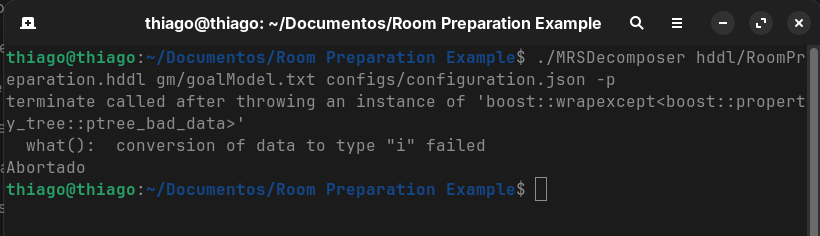
\includegraphics[width=1\textwidth]{erro_mutrose.png} 
    \caption{}
  \end{figure}
\end{frame}

\section{Desenvolvimento}
\begin{frame}{Flows}
  \begin{figure}[!h]
    \centering
    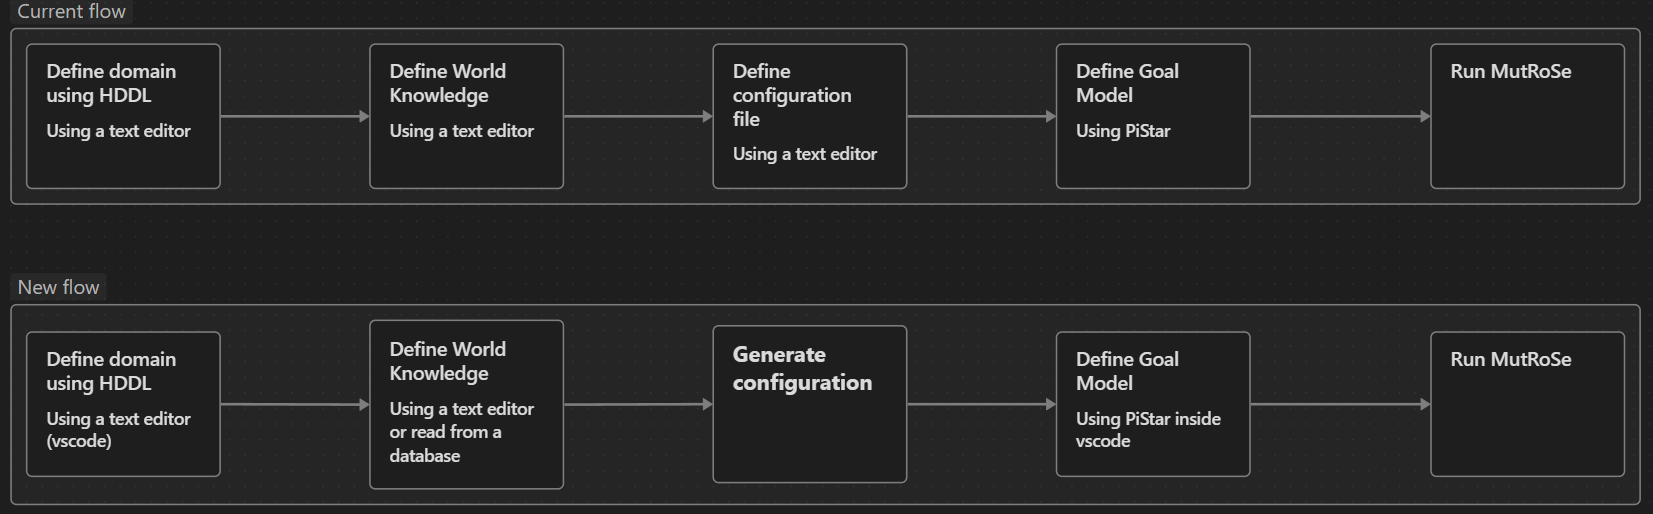
\includegraphics[width=1\textwidth]{VSCode extension flows.png} 
    \caption{}
  \end{figure}
\end{frame}
\begin{frame}{A extensão}
  \begin{figure}[!h]
    \centering
    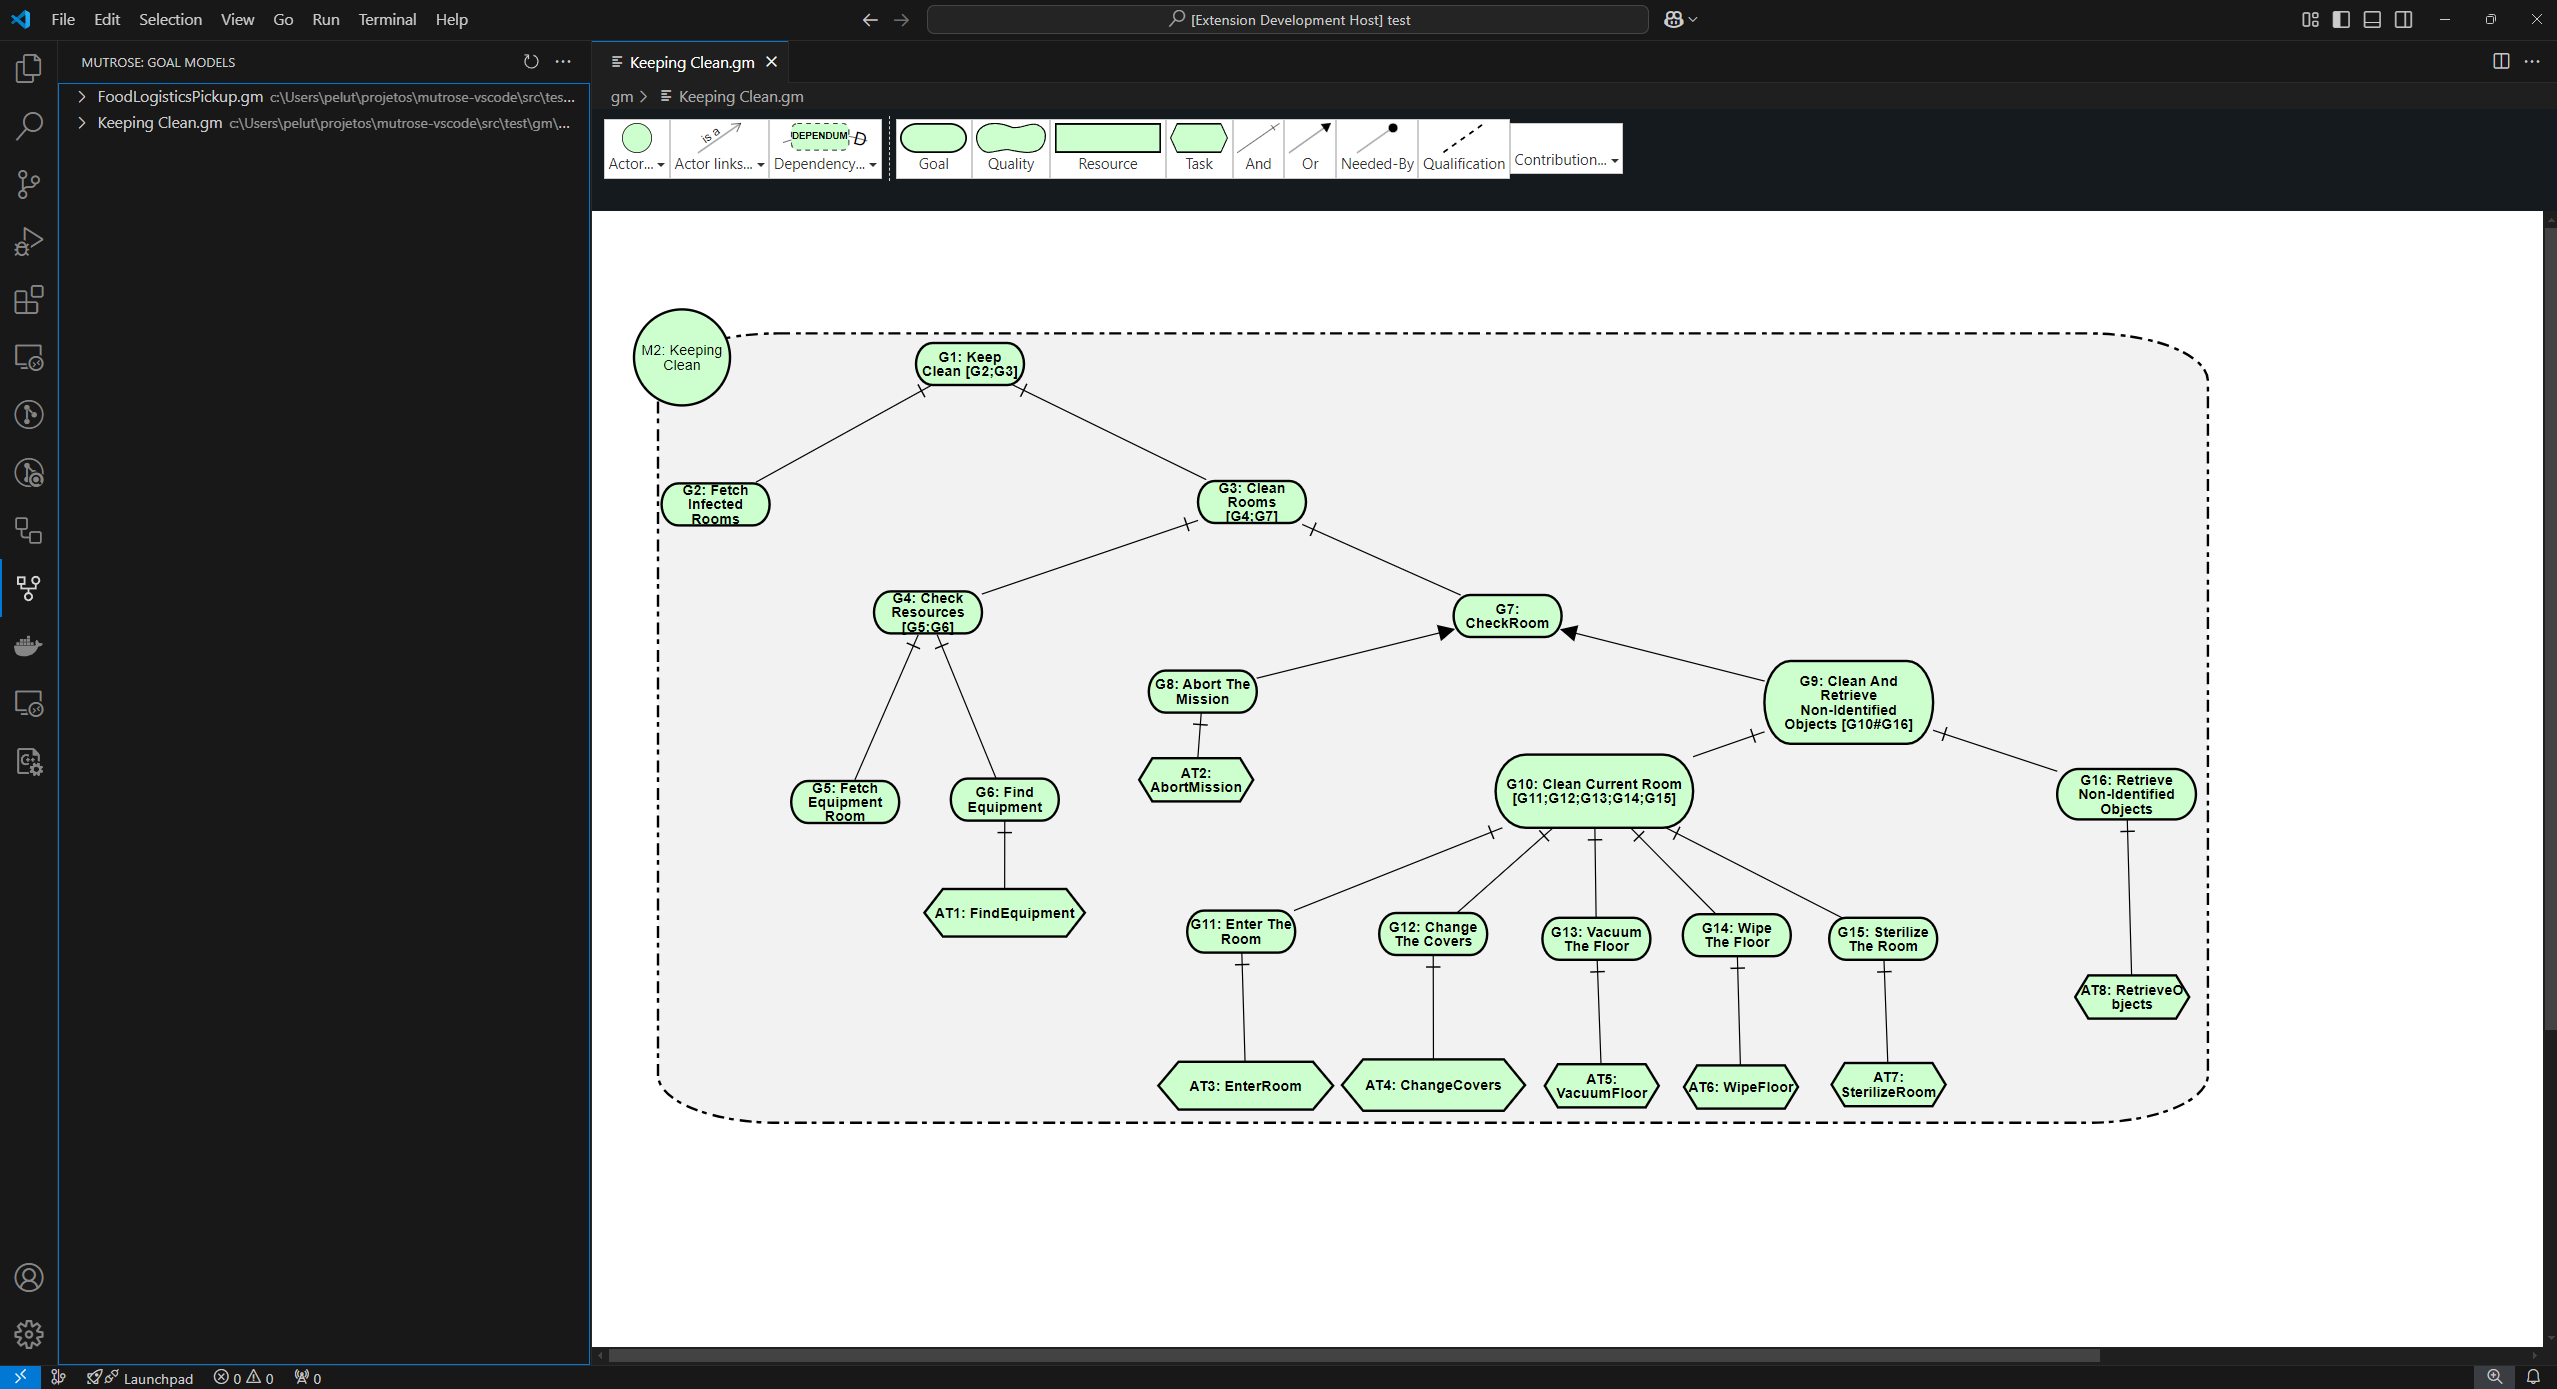
\includegraphics[width=1\textwidth]{vscode print.png} 
    \caption{}
  \end{figure}
\end{frame}

\begin{frame}{Custom Text Editor}
  \begin{figure}[!h]
    \centering
    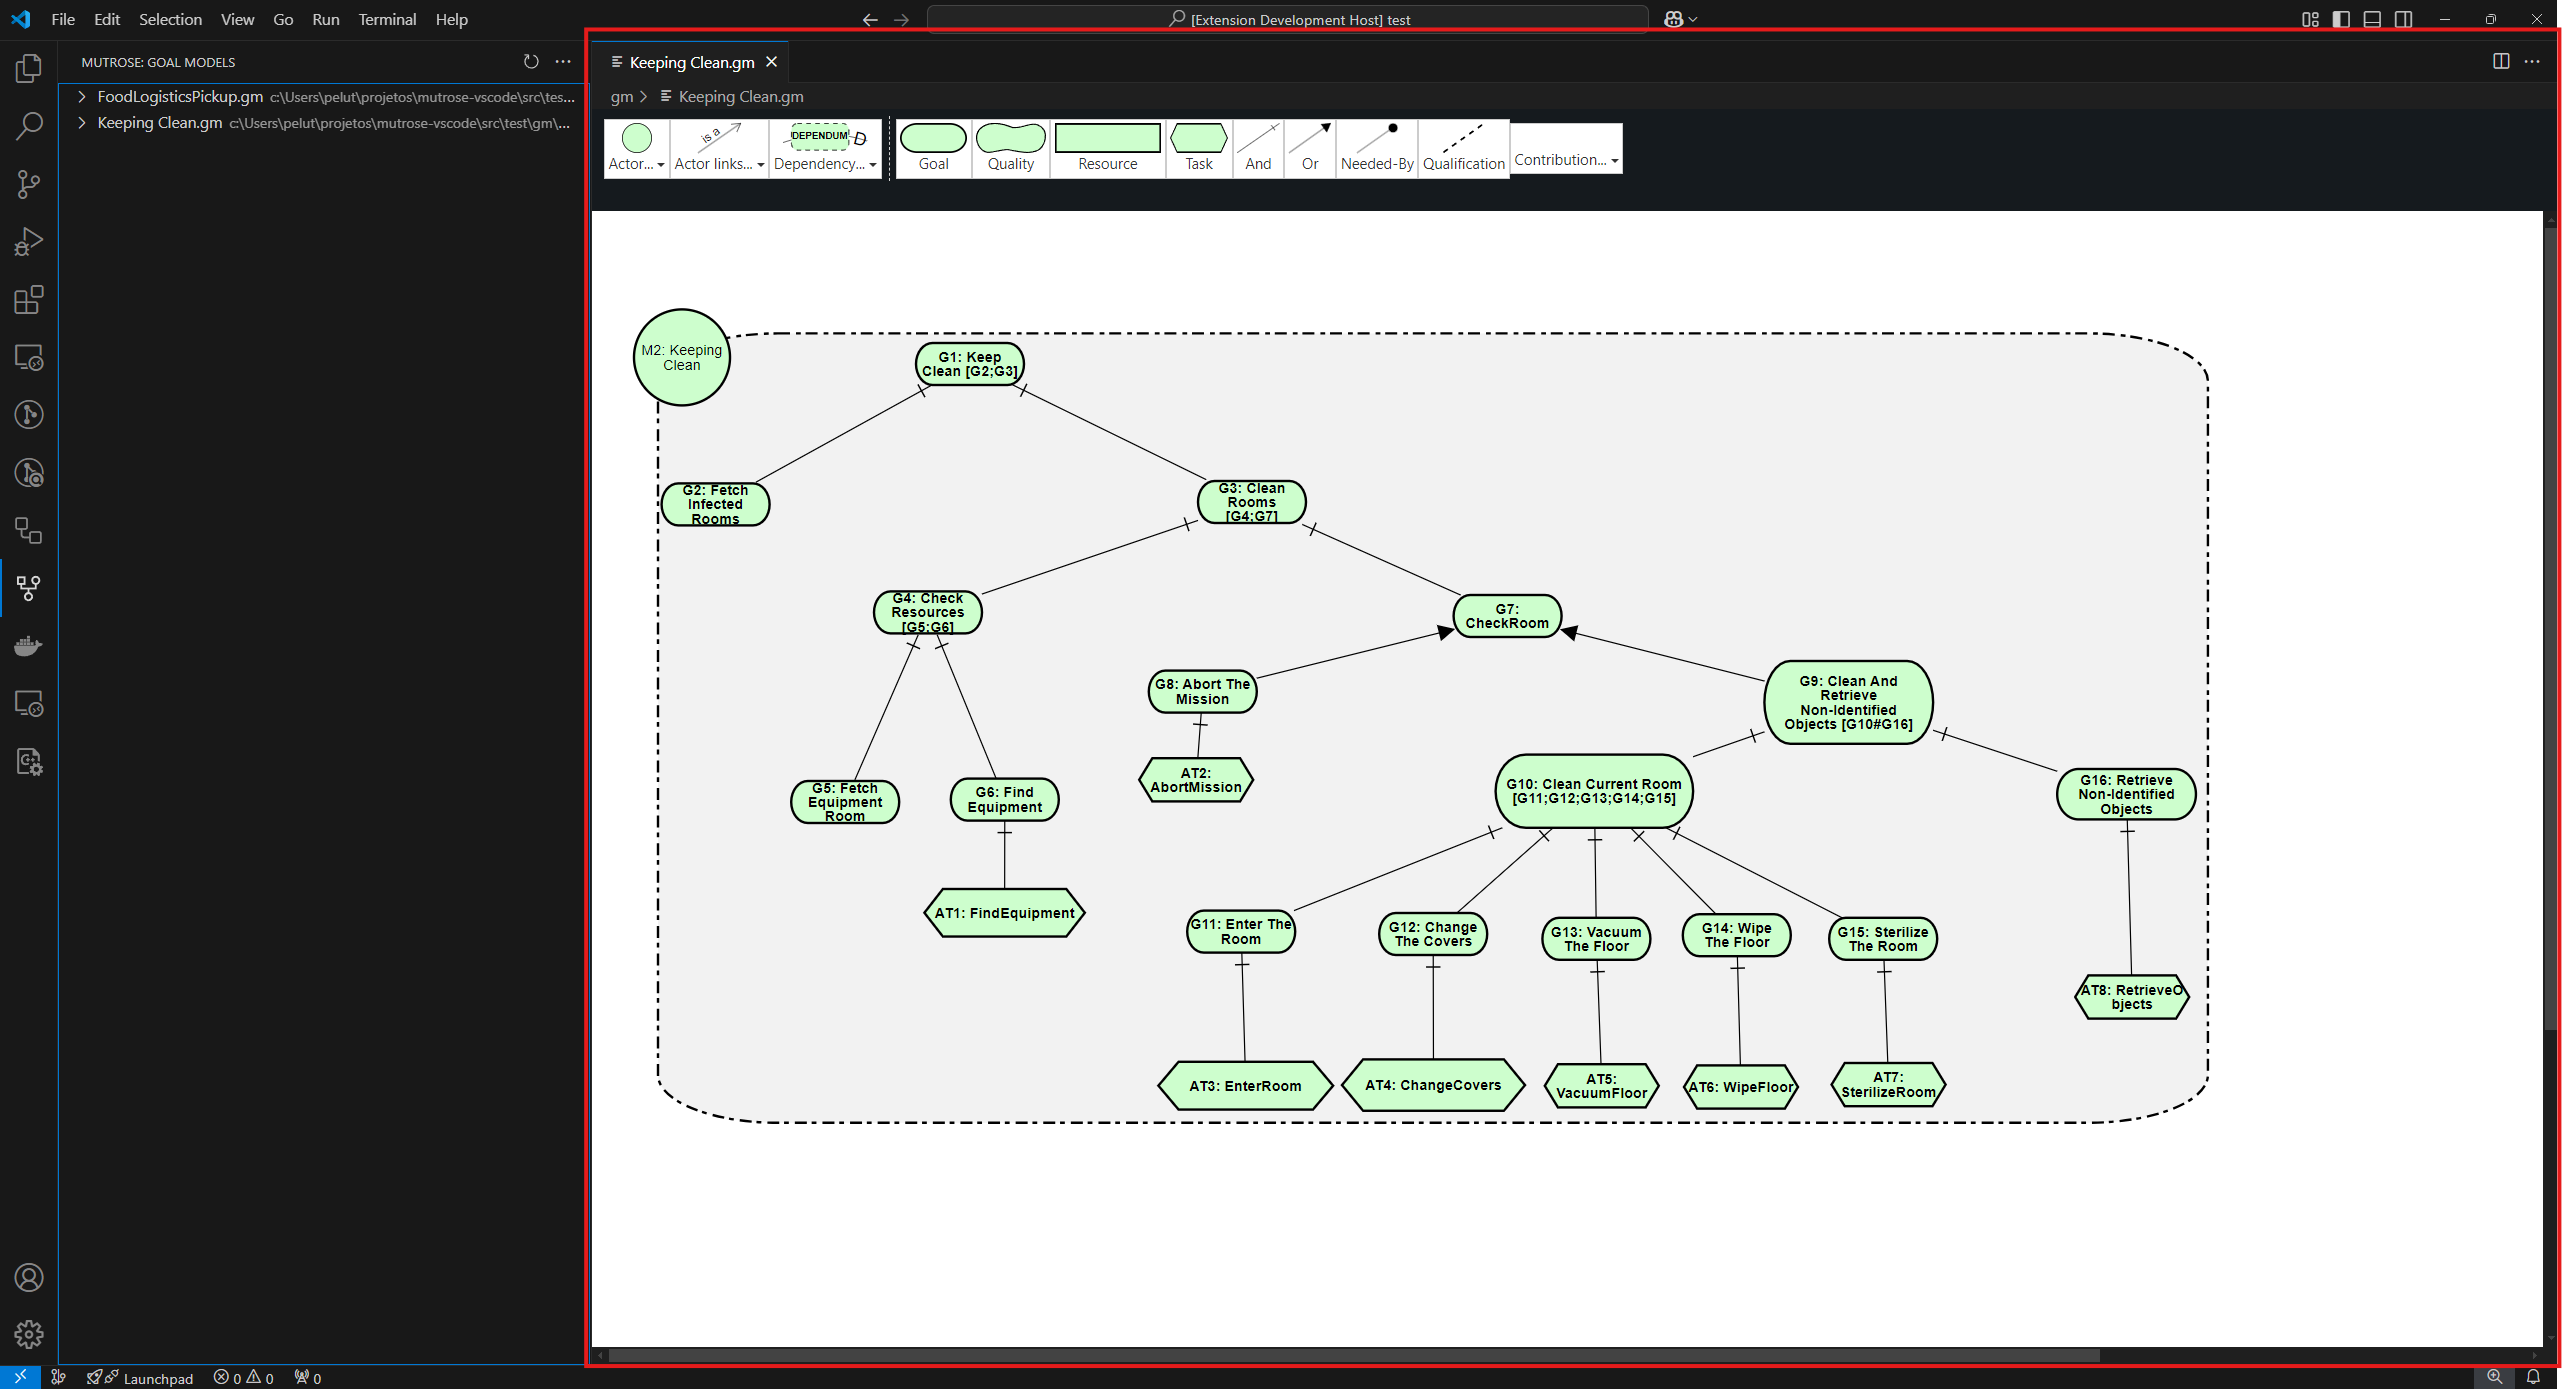
\includegraphics[width=1\textwidth]{custom_texteditor.png} 
    \caption{}
  \end{figure}
\end{frame}
\begin{frame}{Tree View}
  \begin{figure}[!h]
    \centering
    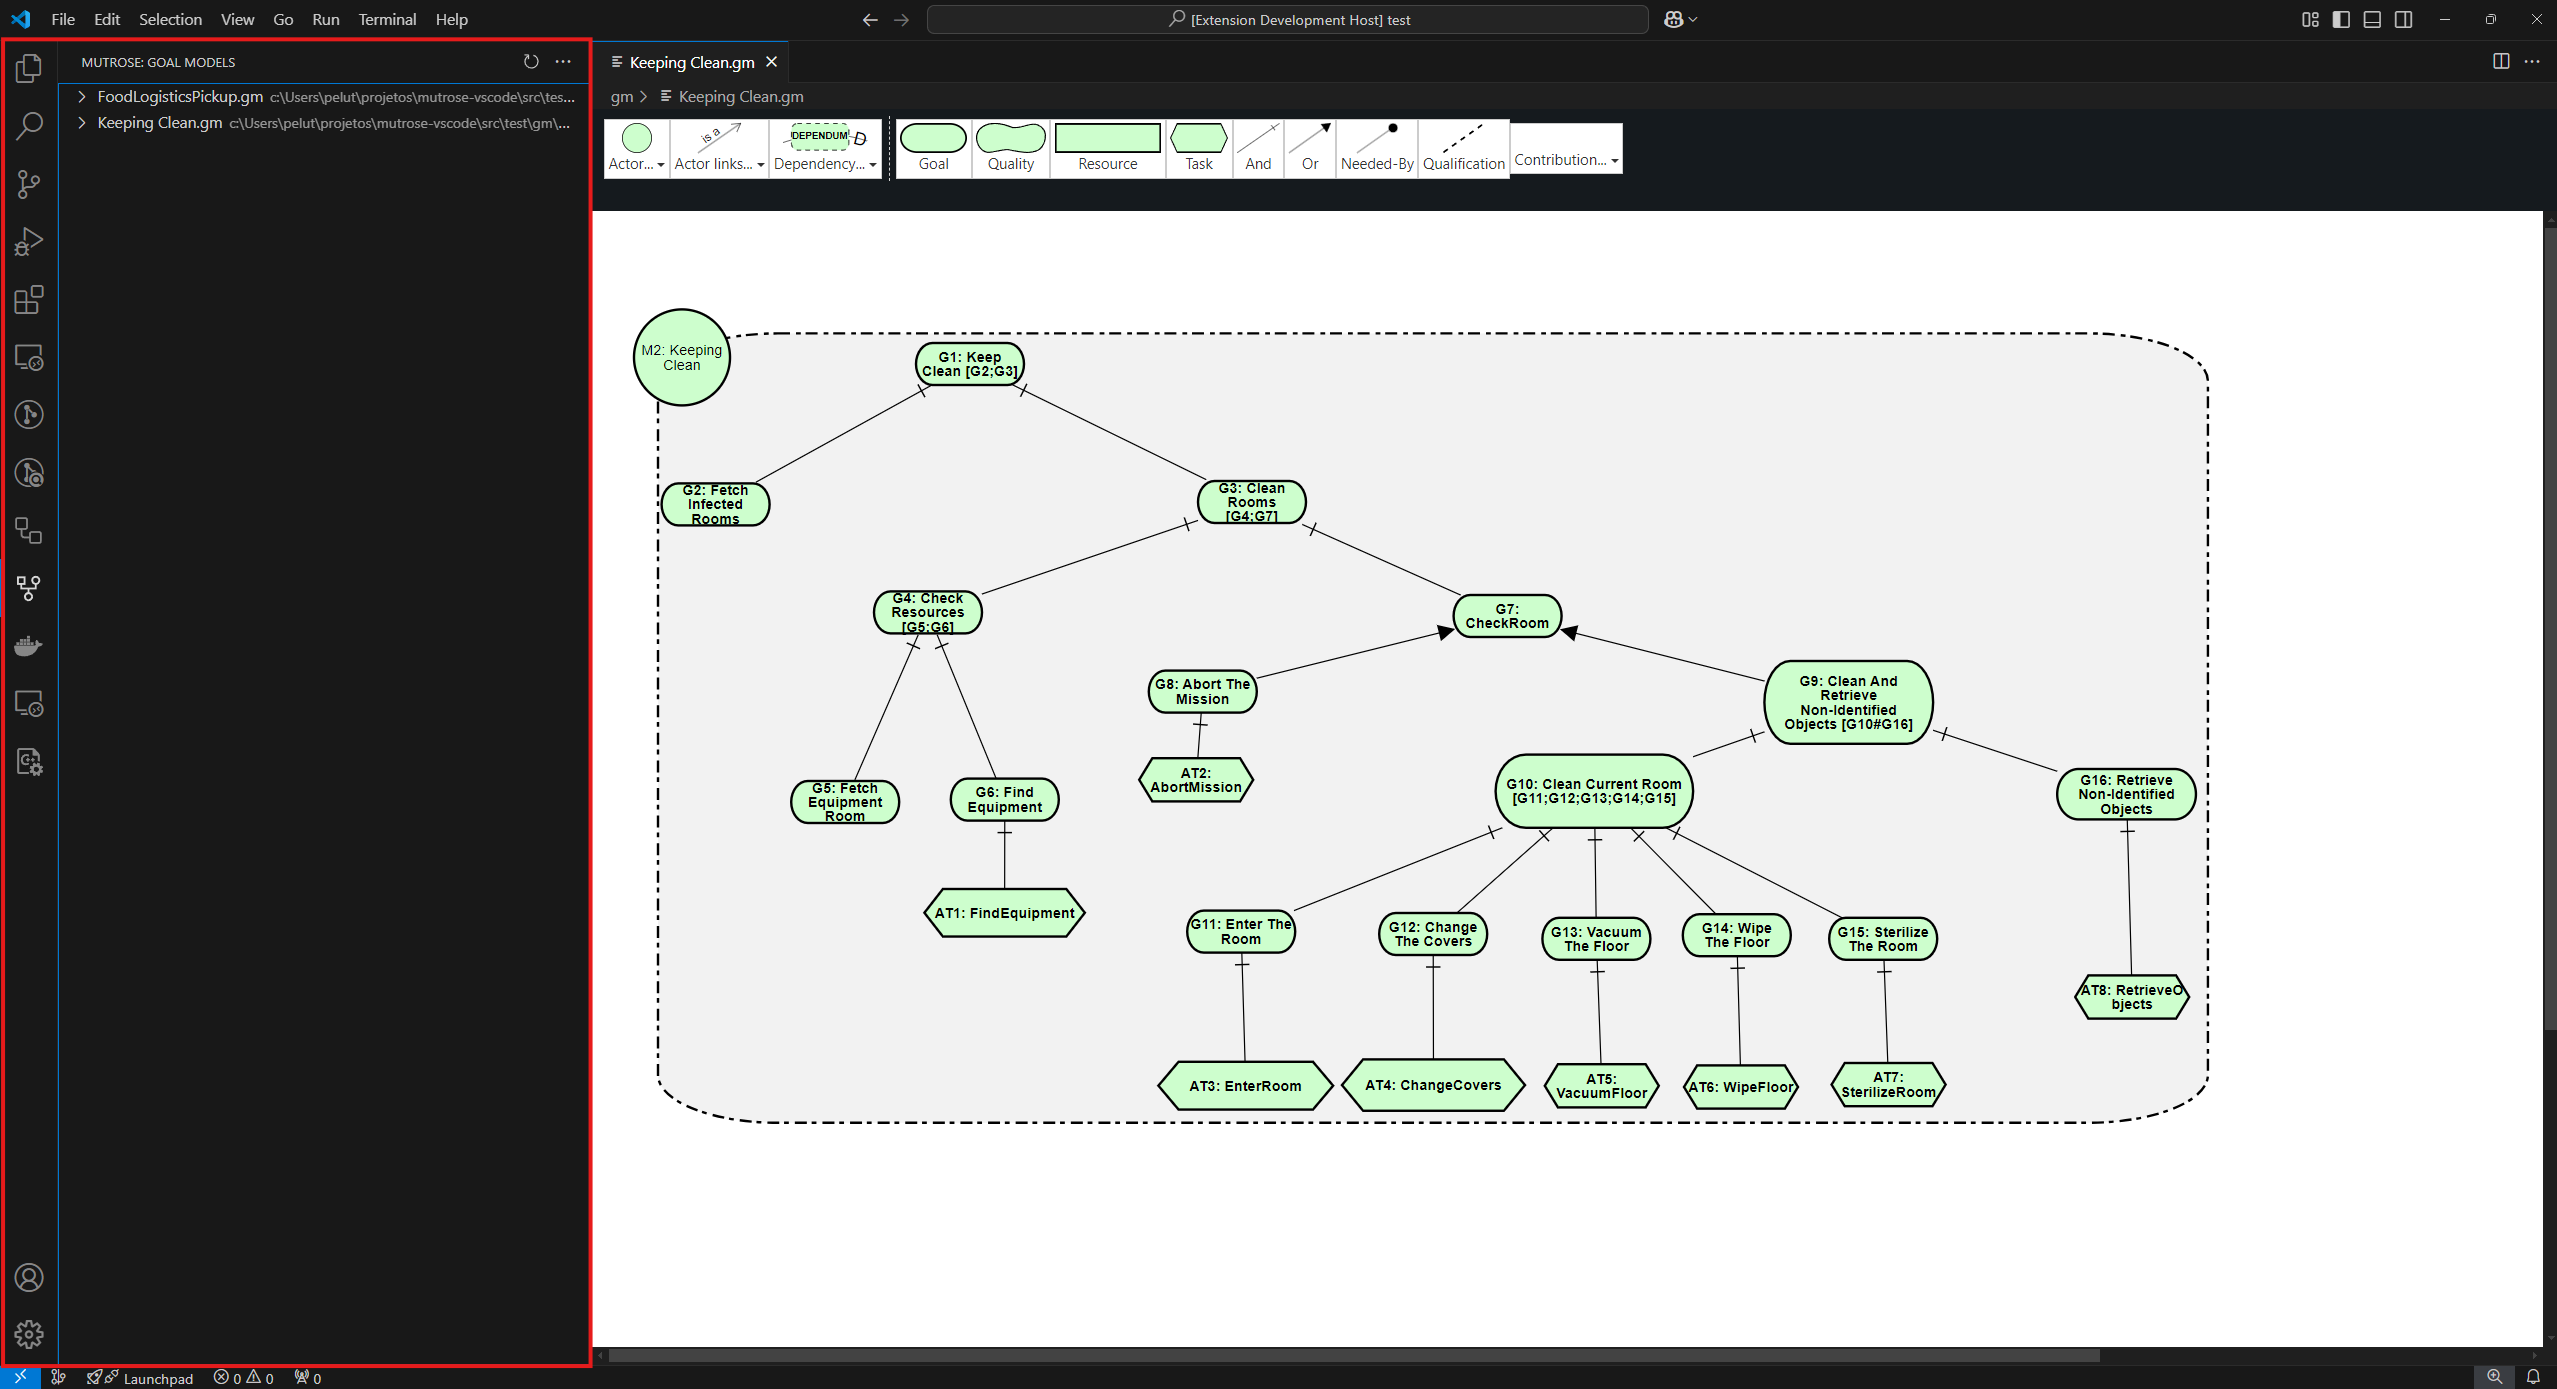
\includegraphics[width=1\textwidth]{treeview.png} 
    \caption{}
  \end{figure}
\end{frame}
\begin{frame}{Tree View nodes}
  \begin{figure}[!h]
    \centering
    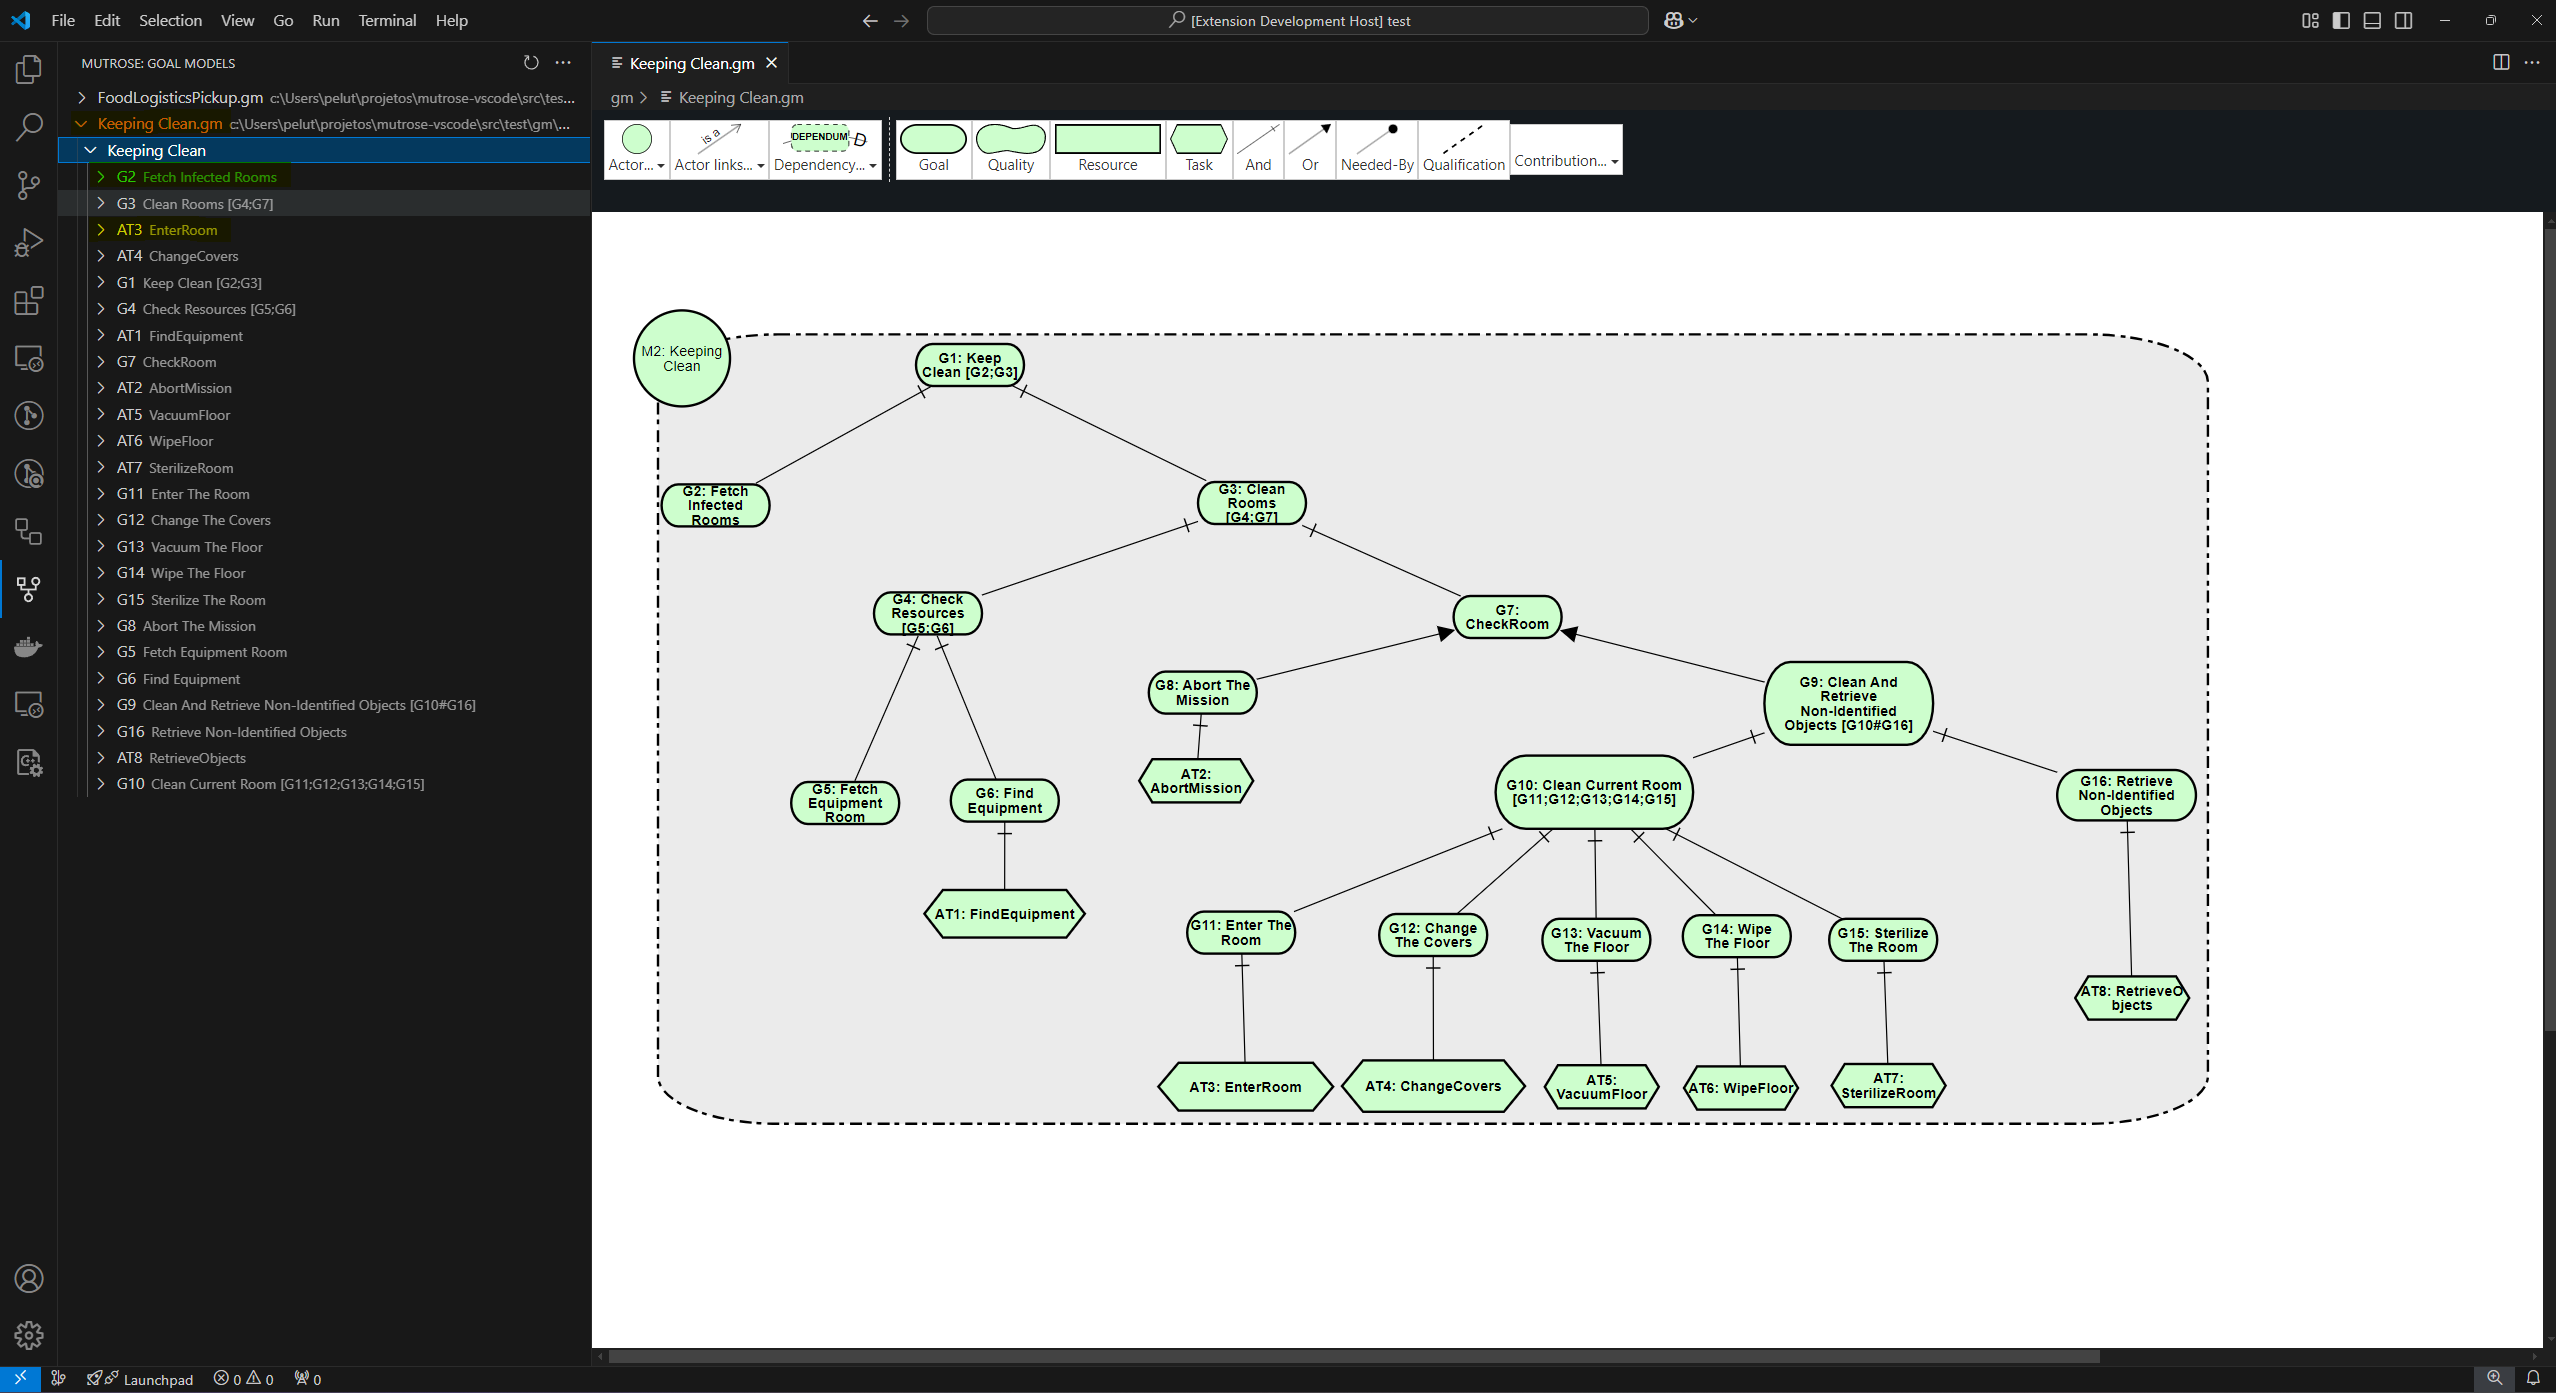
\includegraphics[width=1\textwidth]{Mission in treeview.png} 
    \caption{}
  \end{figure}
\end{frame}
\begin{frame}{Mission na Tree View}
  \begin{figure}[!h]
    \centering
    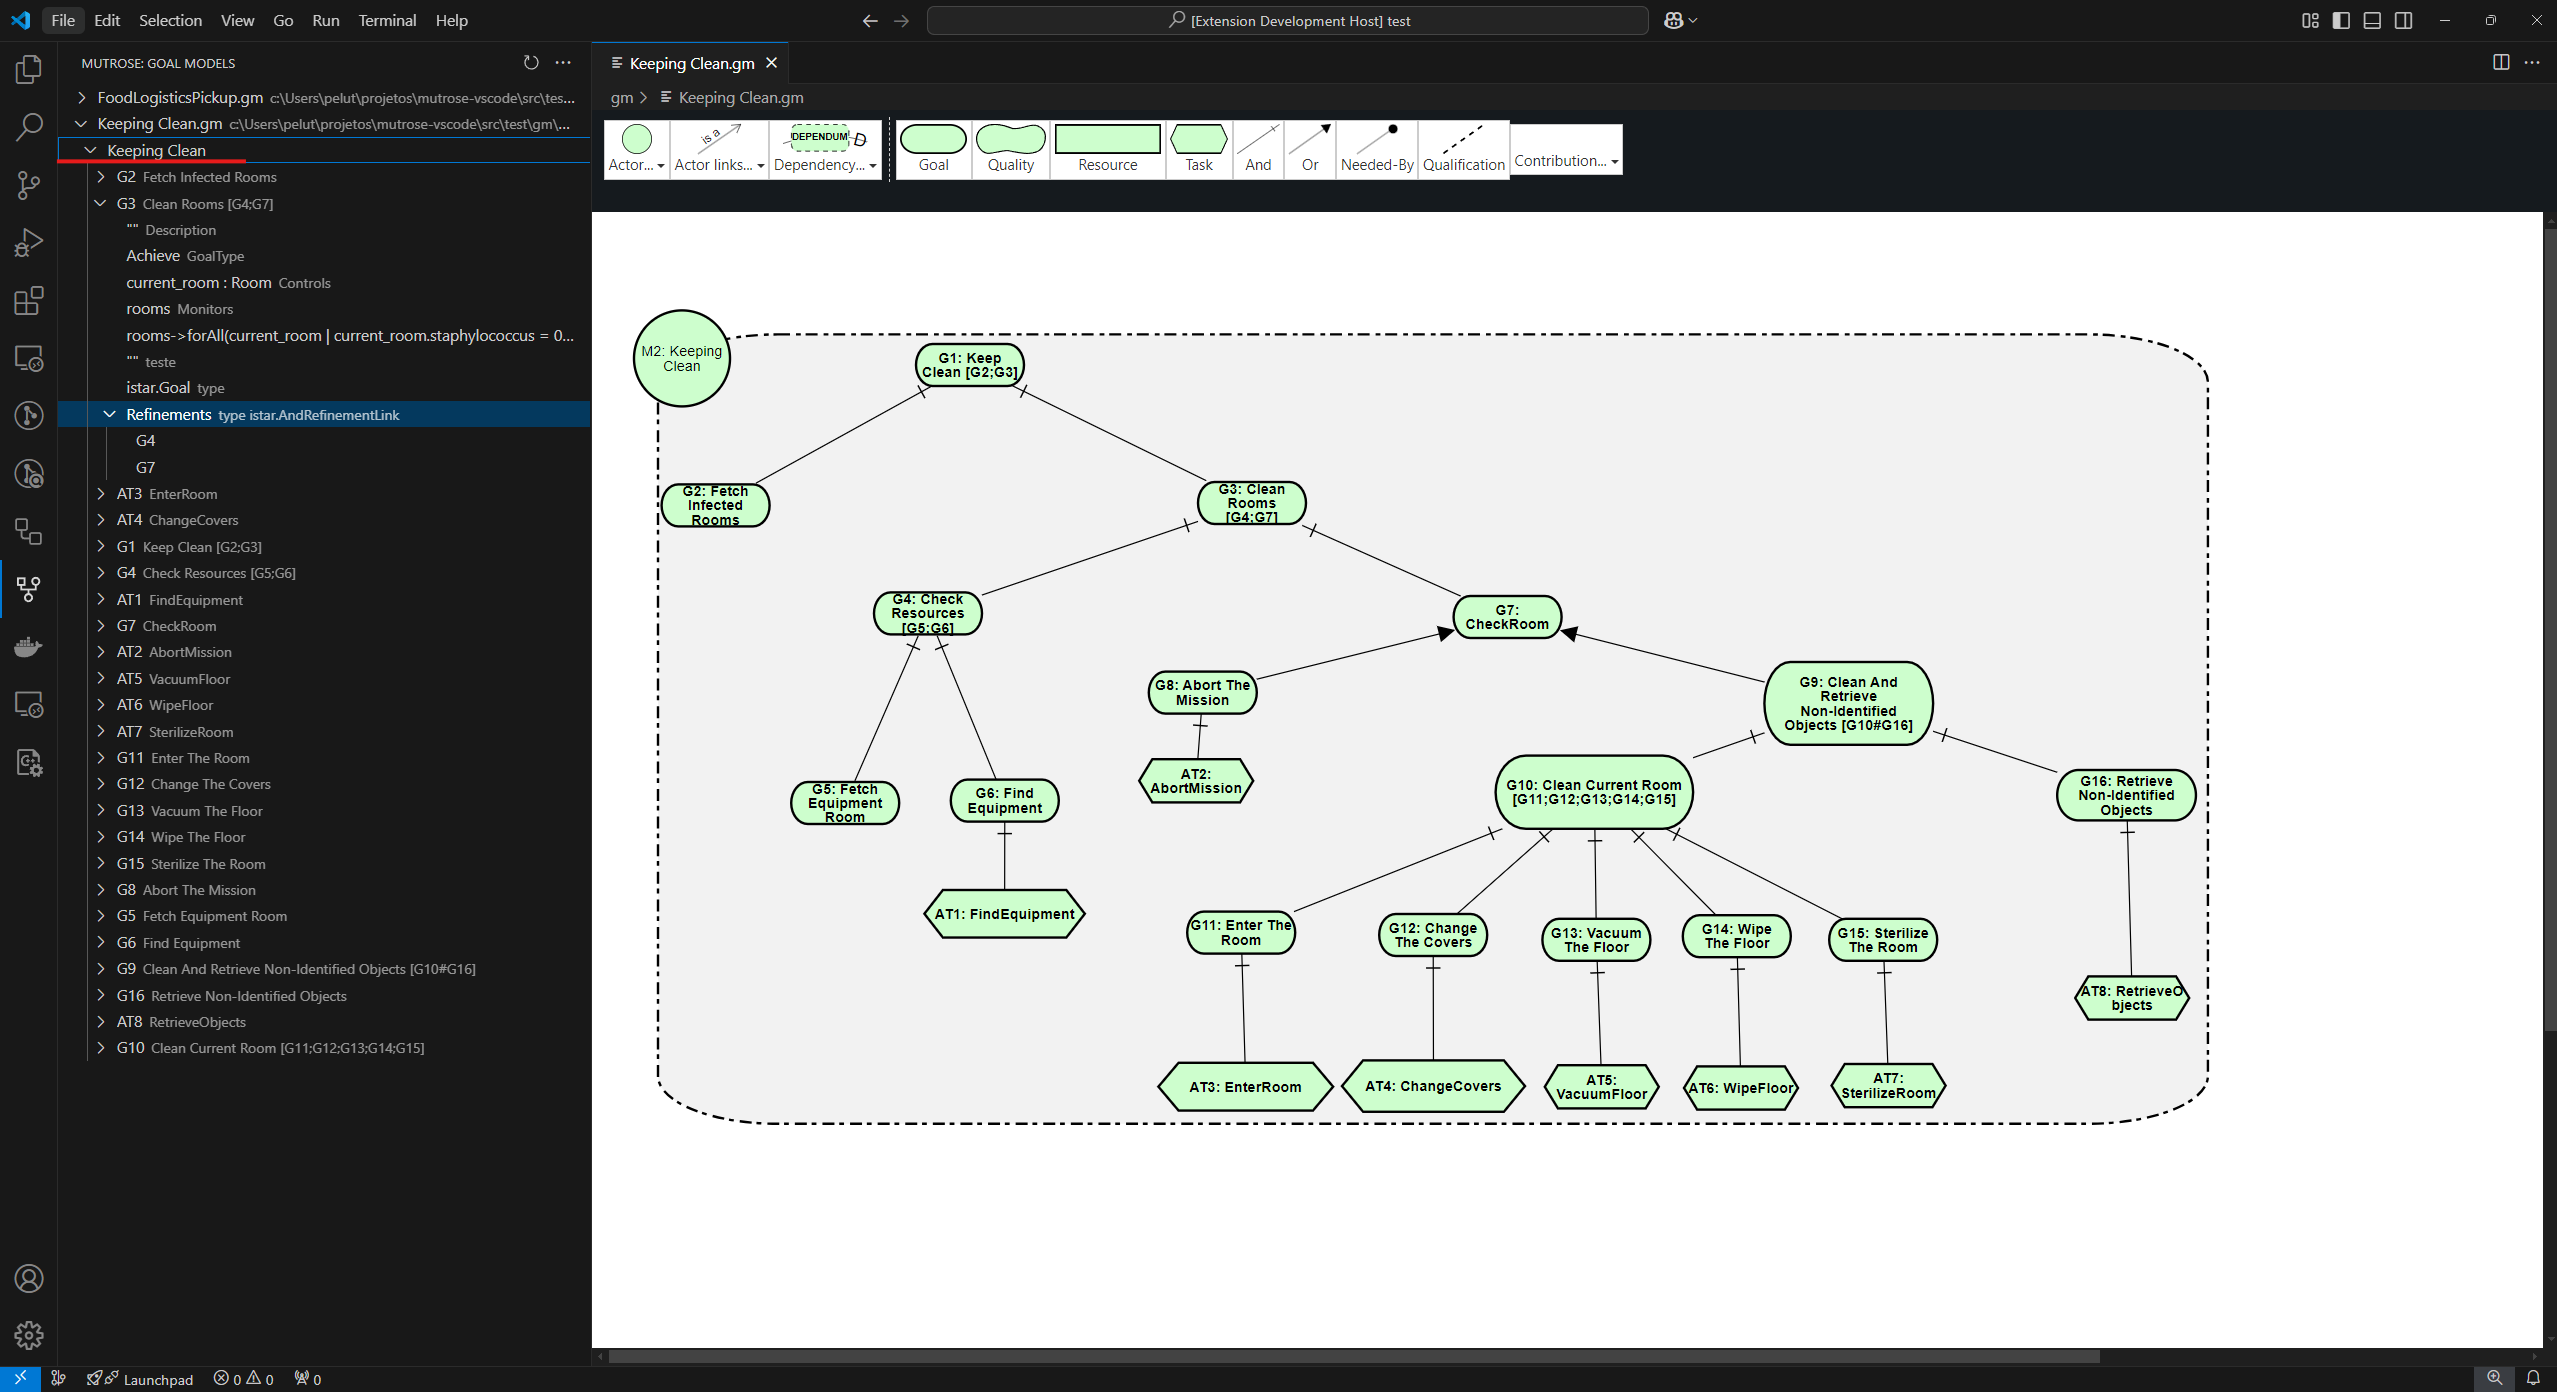
\includegraphics[width=1\textwidth]{missionfocus.png} 
    \caption{}
  \end{figure}
\end{frame}
\begin{frame}{Goal Properties na Tree View}
  \begin{figure}[!h]
    \centering
    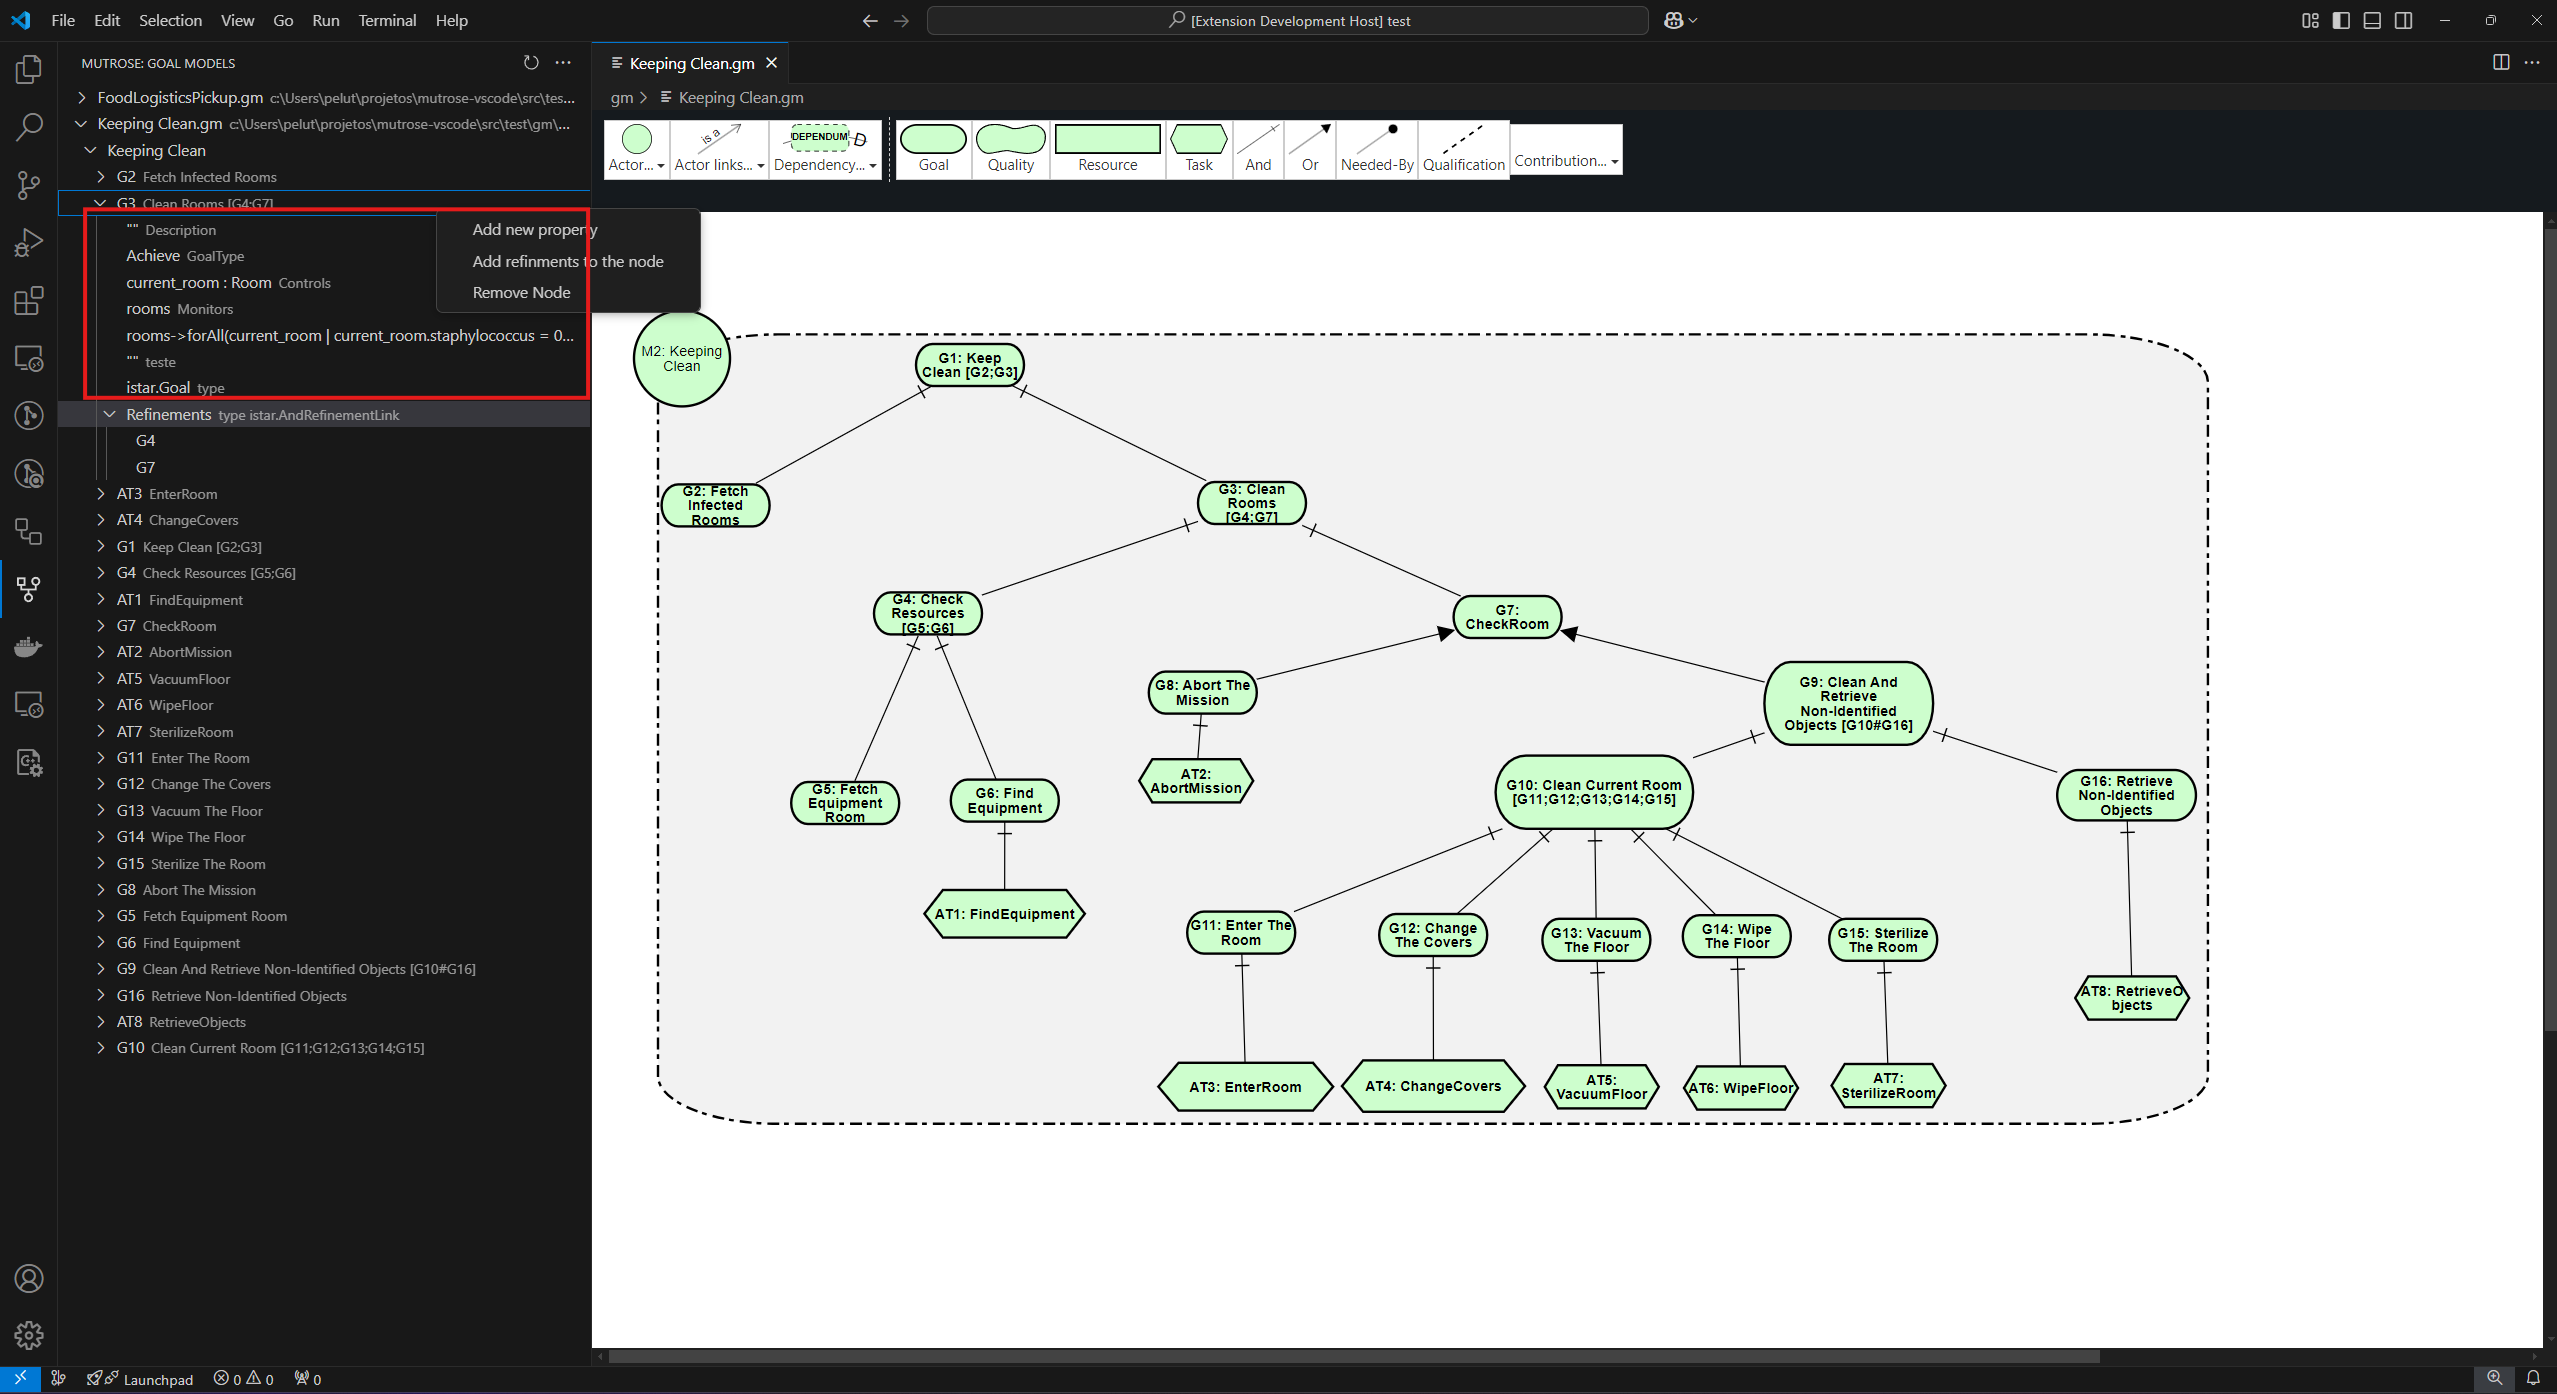
\includegraphics[width=1\textwidth]{node properties.png} 
    \caption{}
  \end{figure}
\end{frame}
\begin{frame}{Refinements na Tree View}
  \begin{figure}[!h]
    \centering
    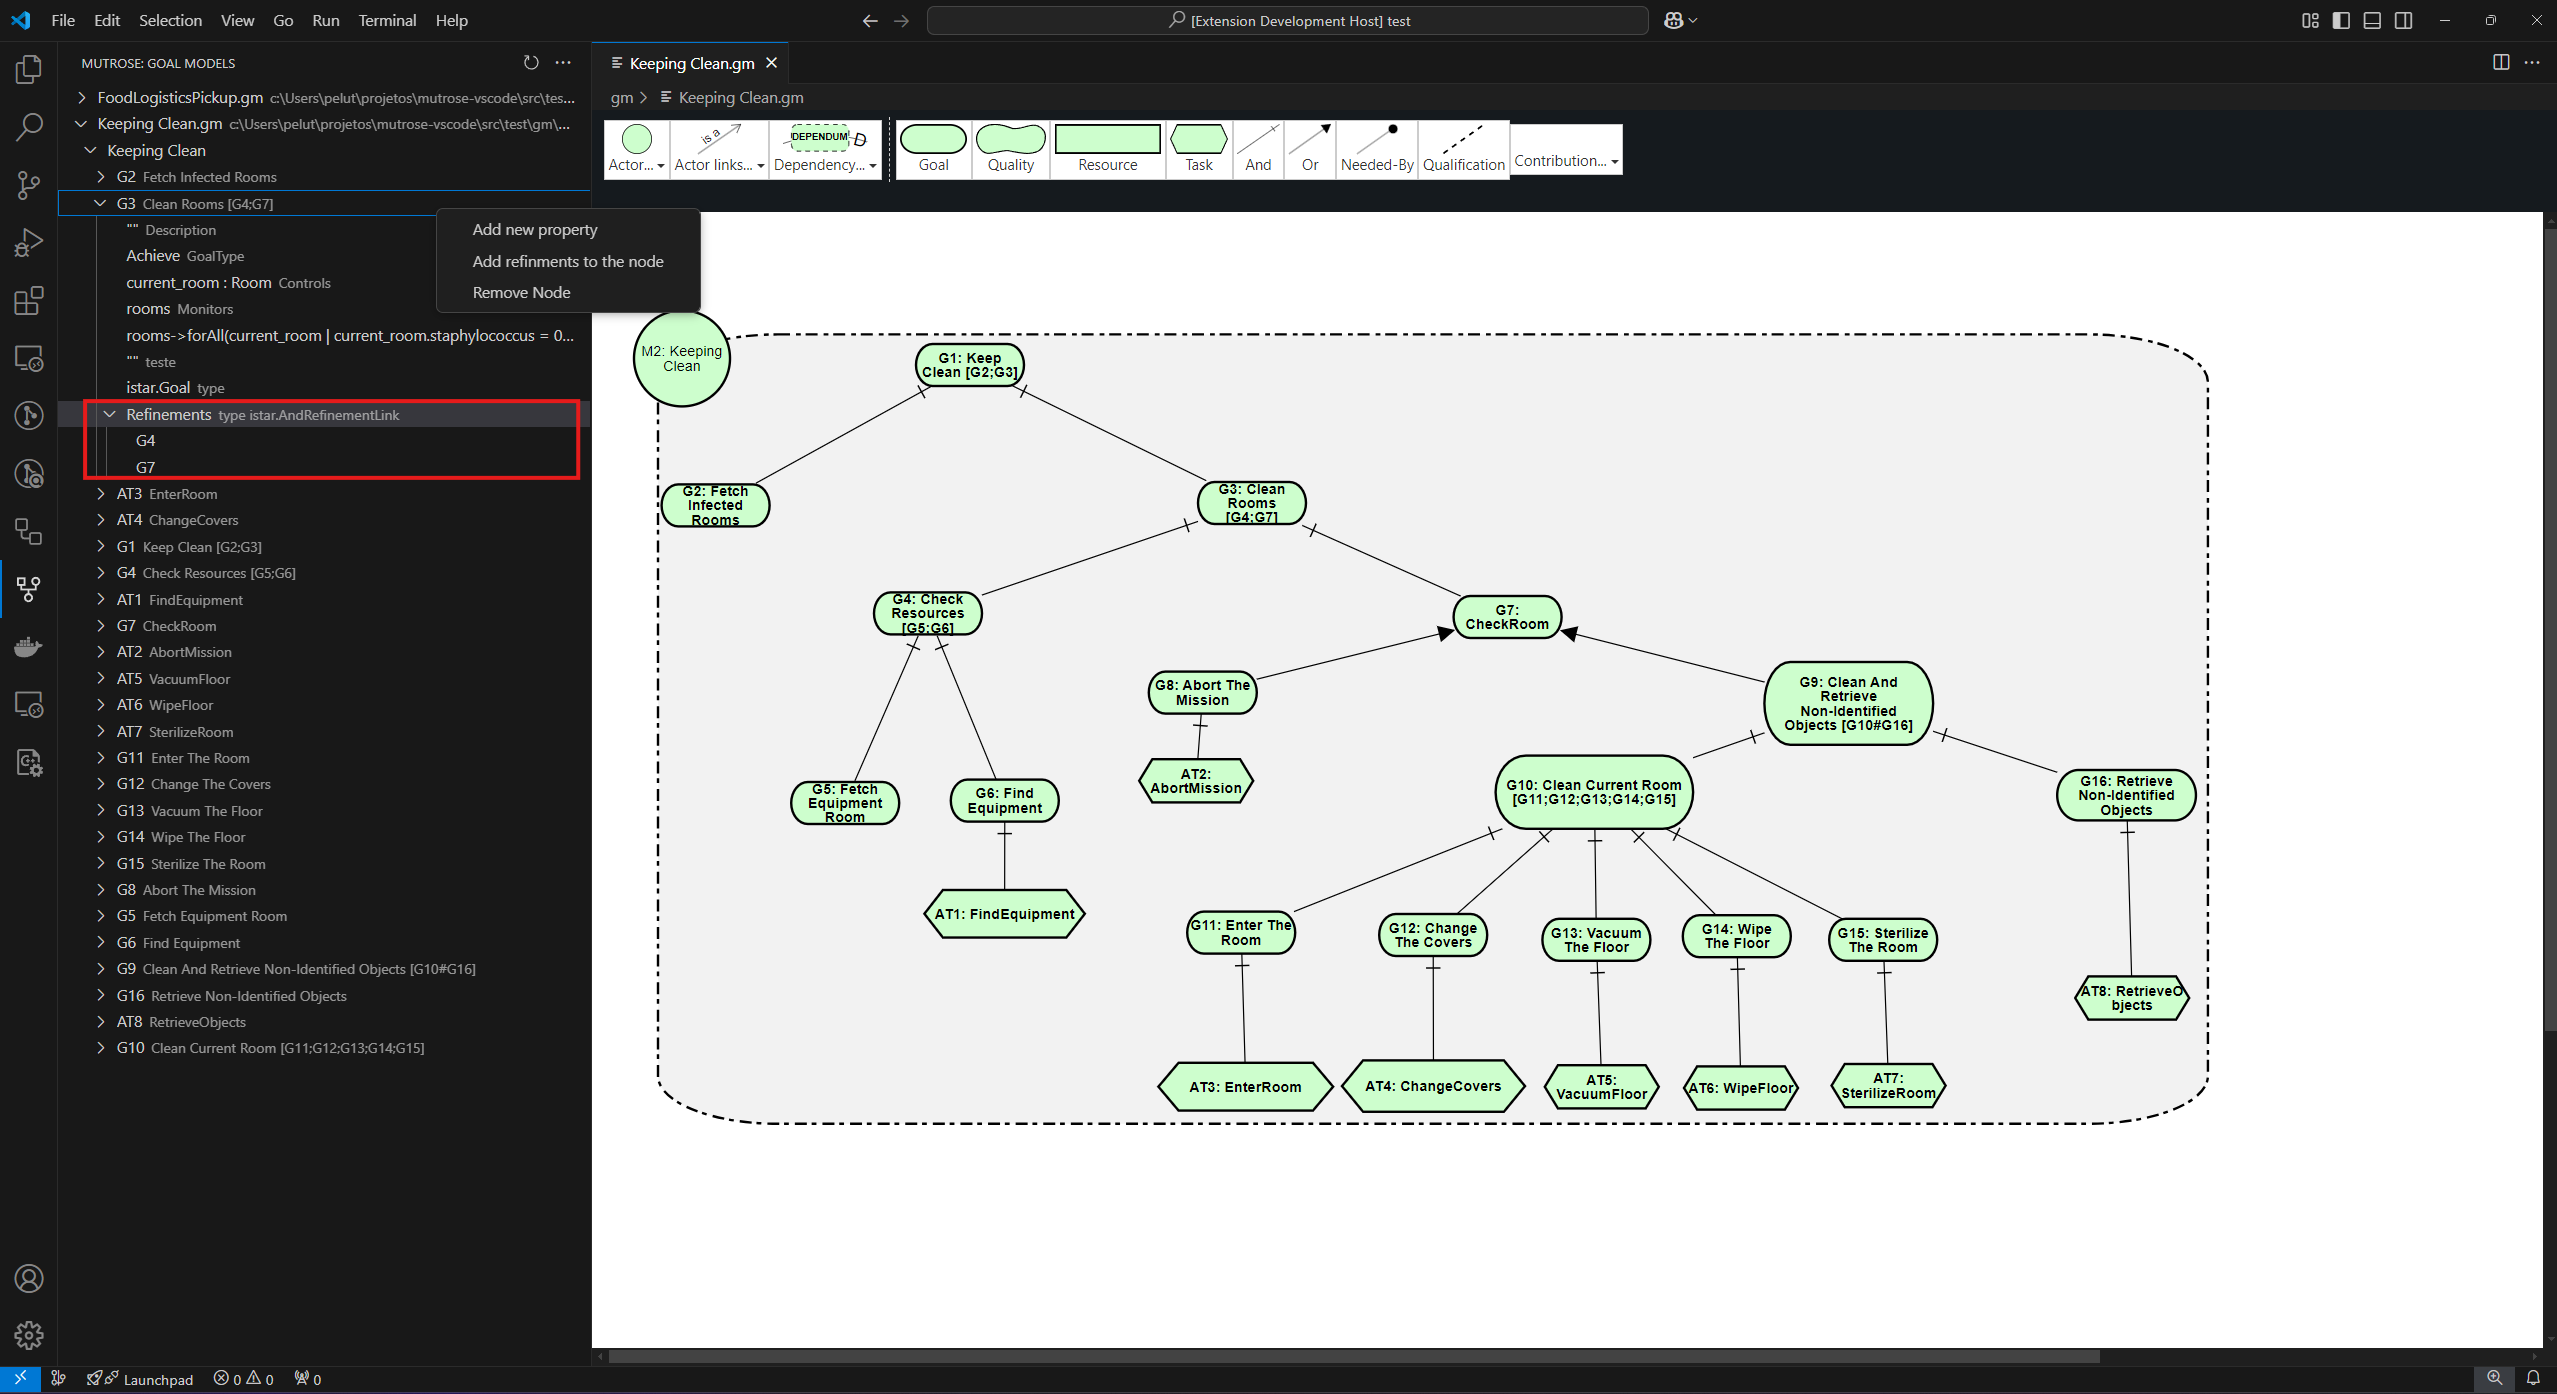
\includegraphics[width=1\textwidth]{refinements.png} 
    \caption{}
  \end{figure}
\end{frame}
\begin{frame}{Context menu do Goal na Tree View}
  \begin{figure}[!h]
    \centering
    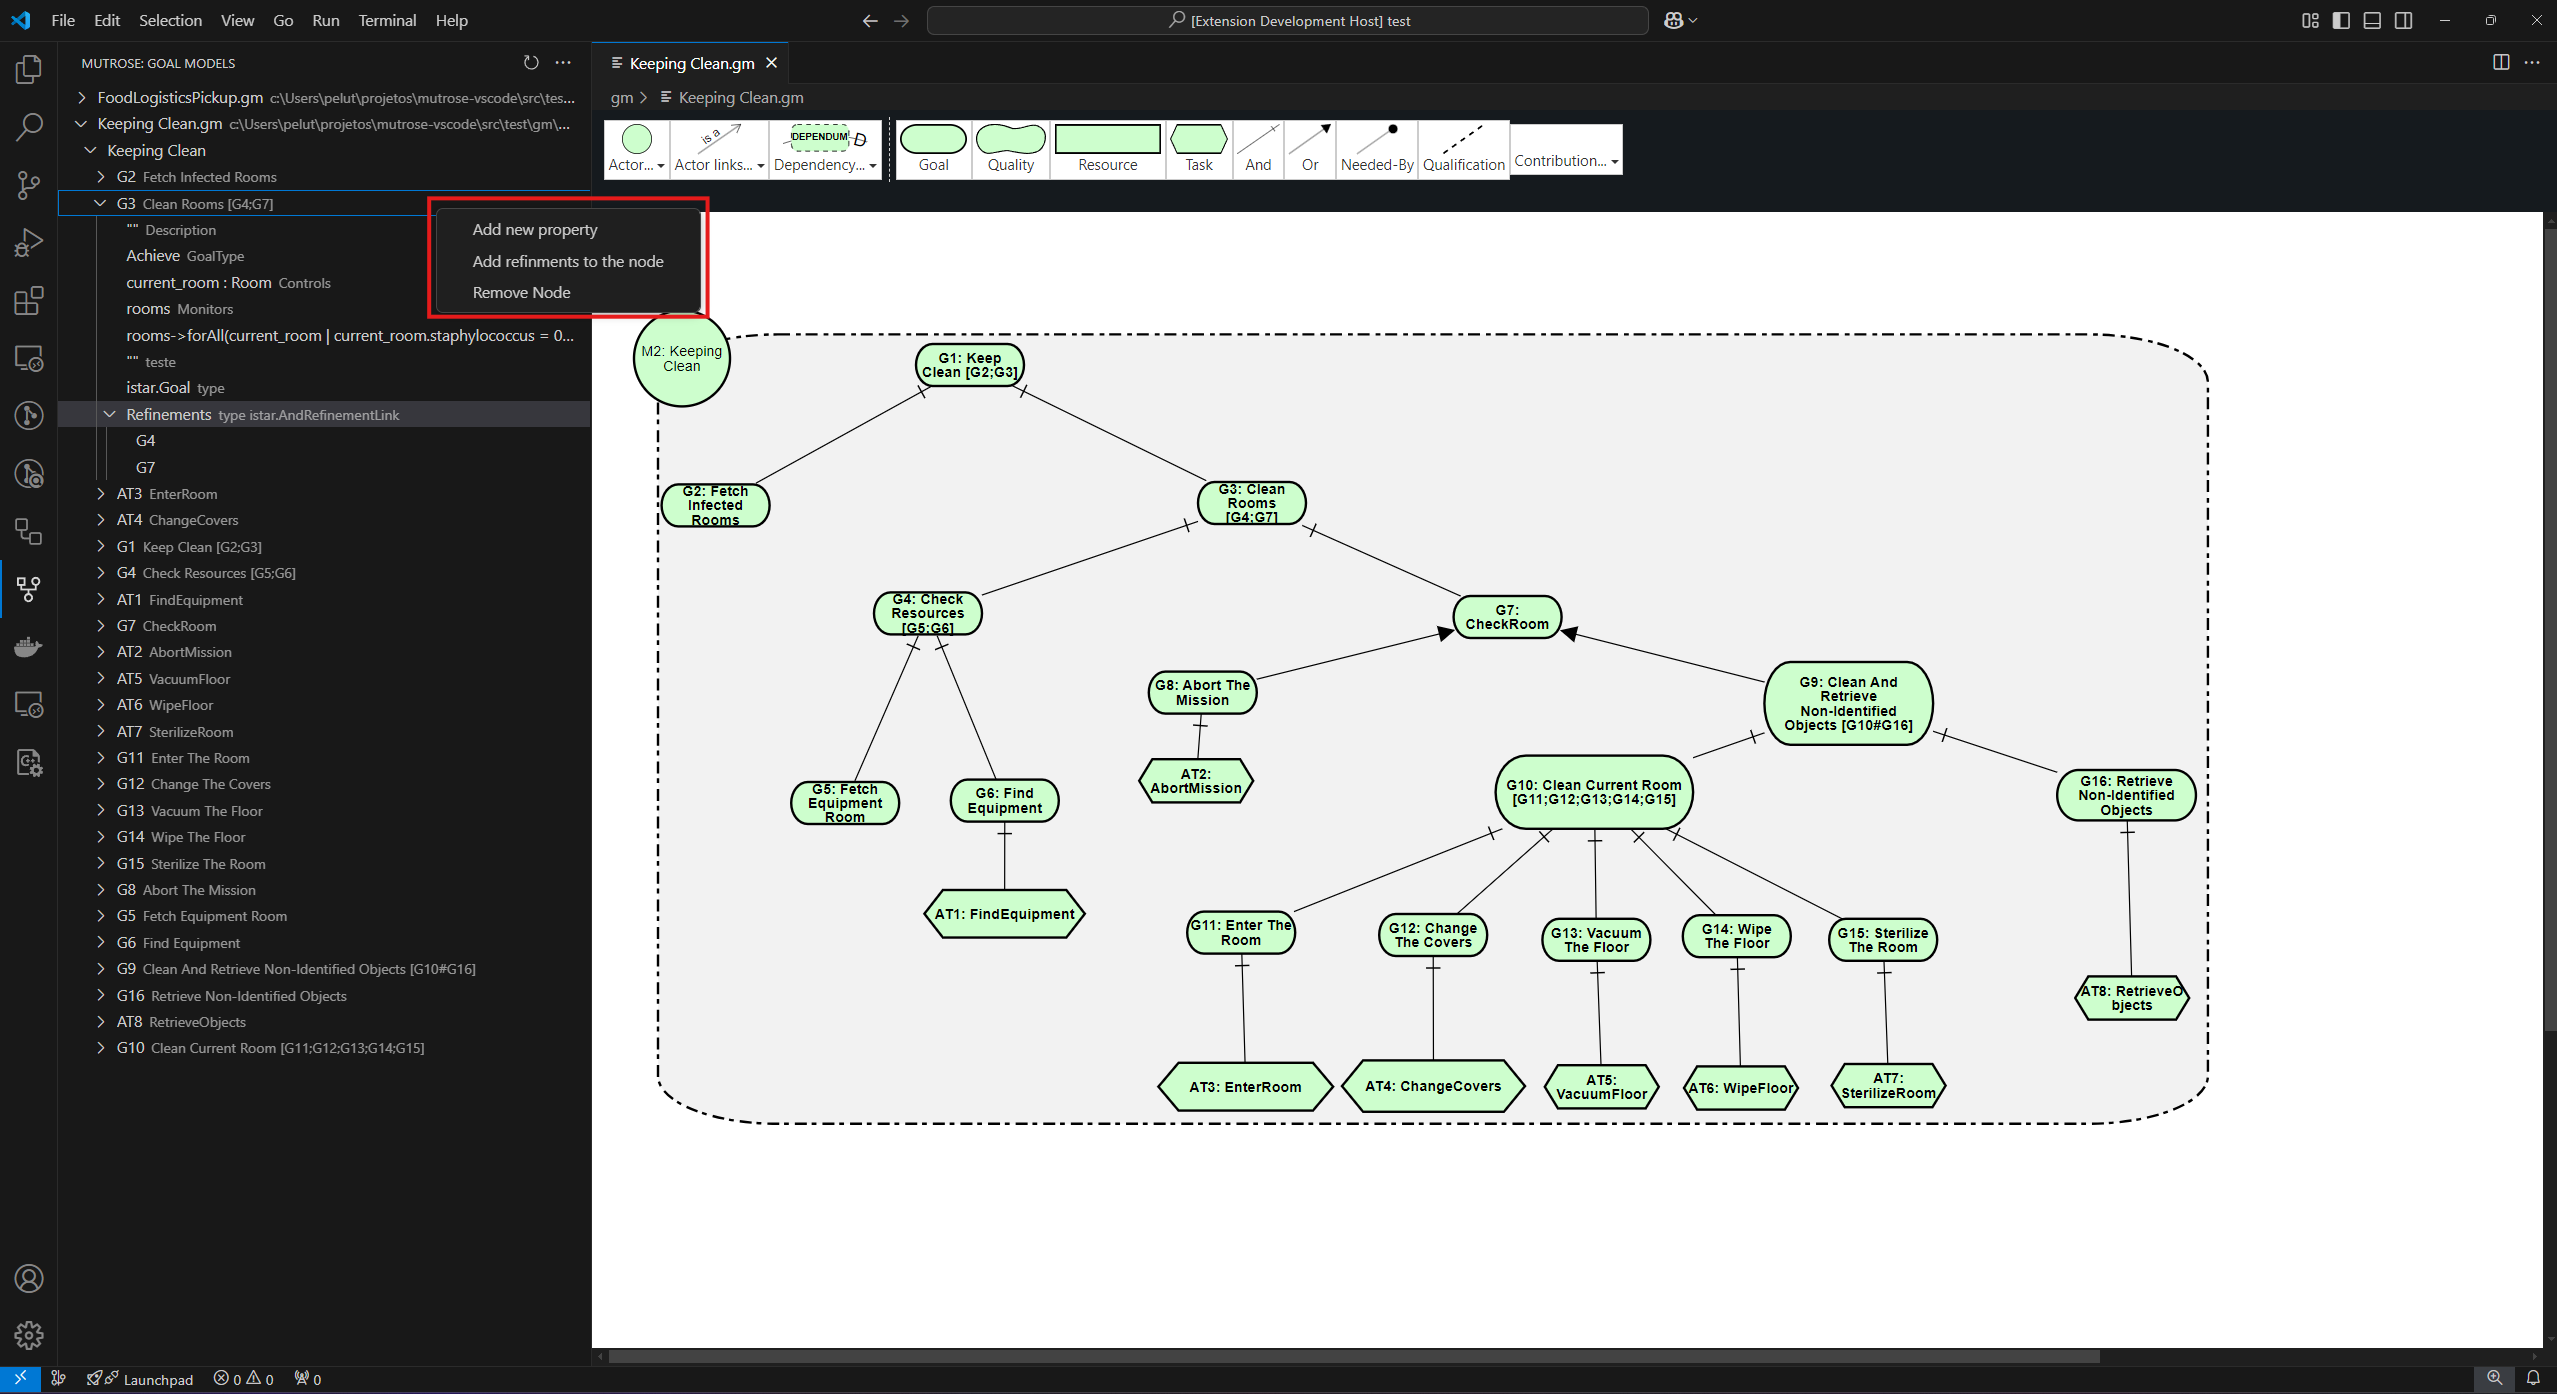
\includegraphics[width=1\textwidth]{submenu_on_right_click.png} 
    \caption{}
  \end{figure}
\end{frame}
\begin{frame}{Context menu da missão na Tree View}
  \begin{figure}[!h]
    \centering
    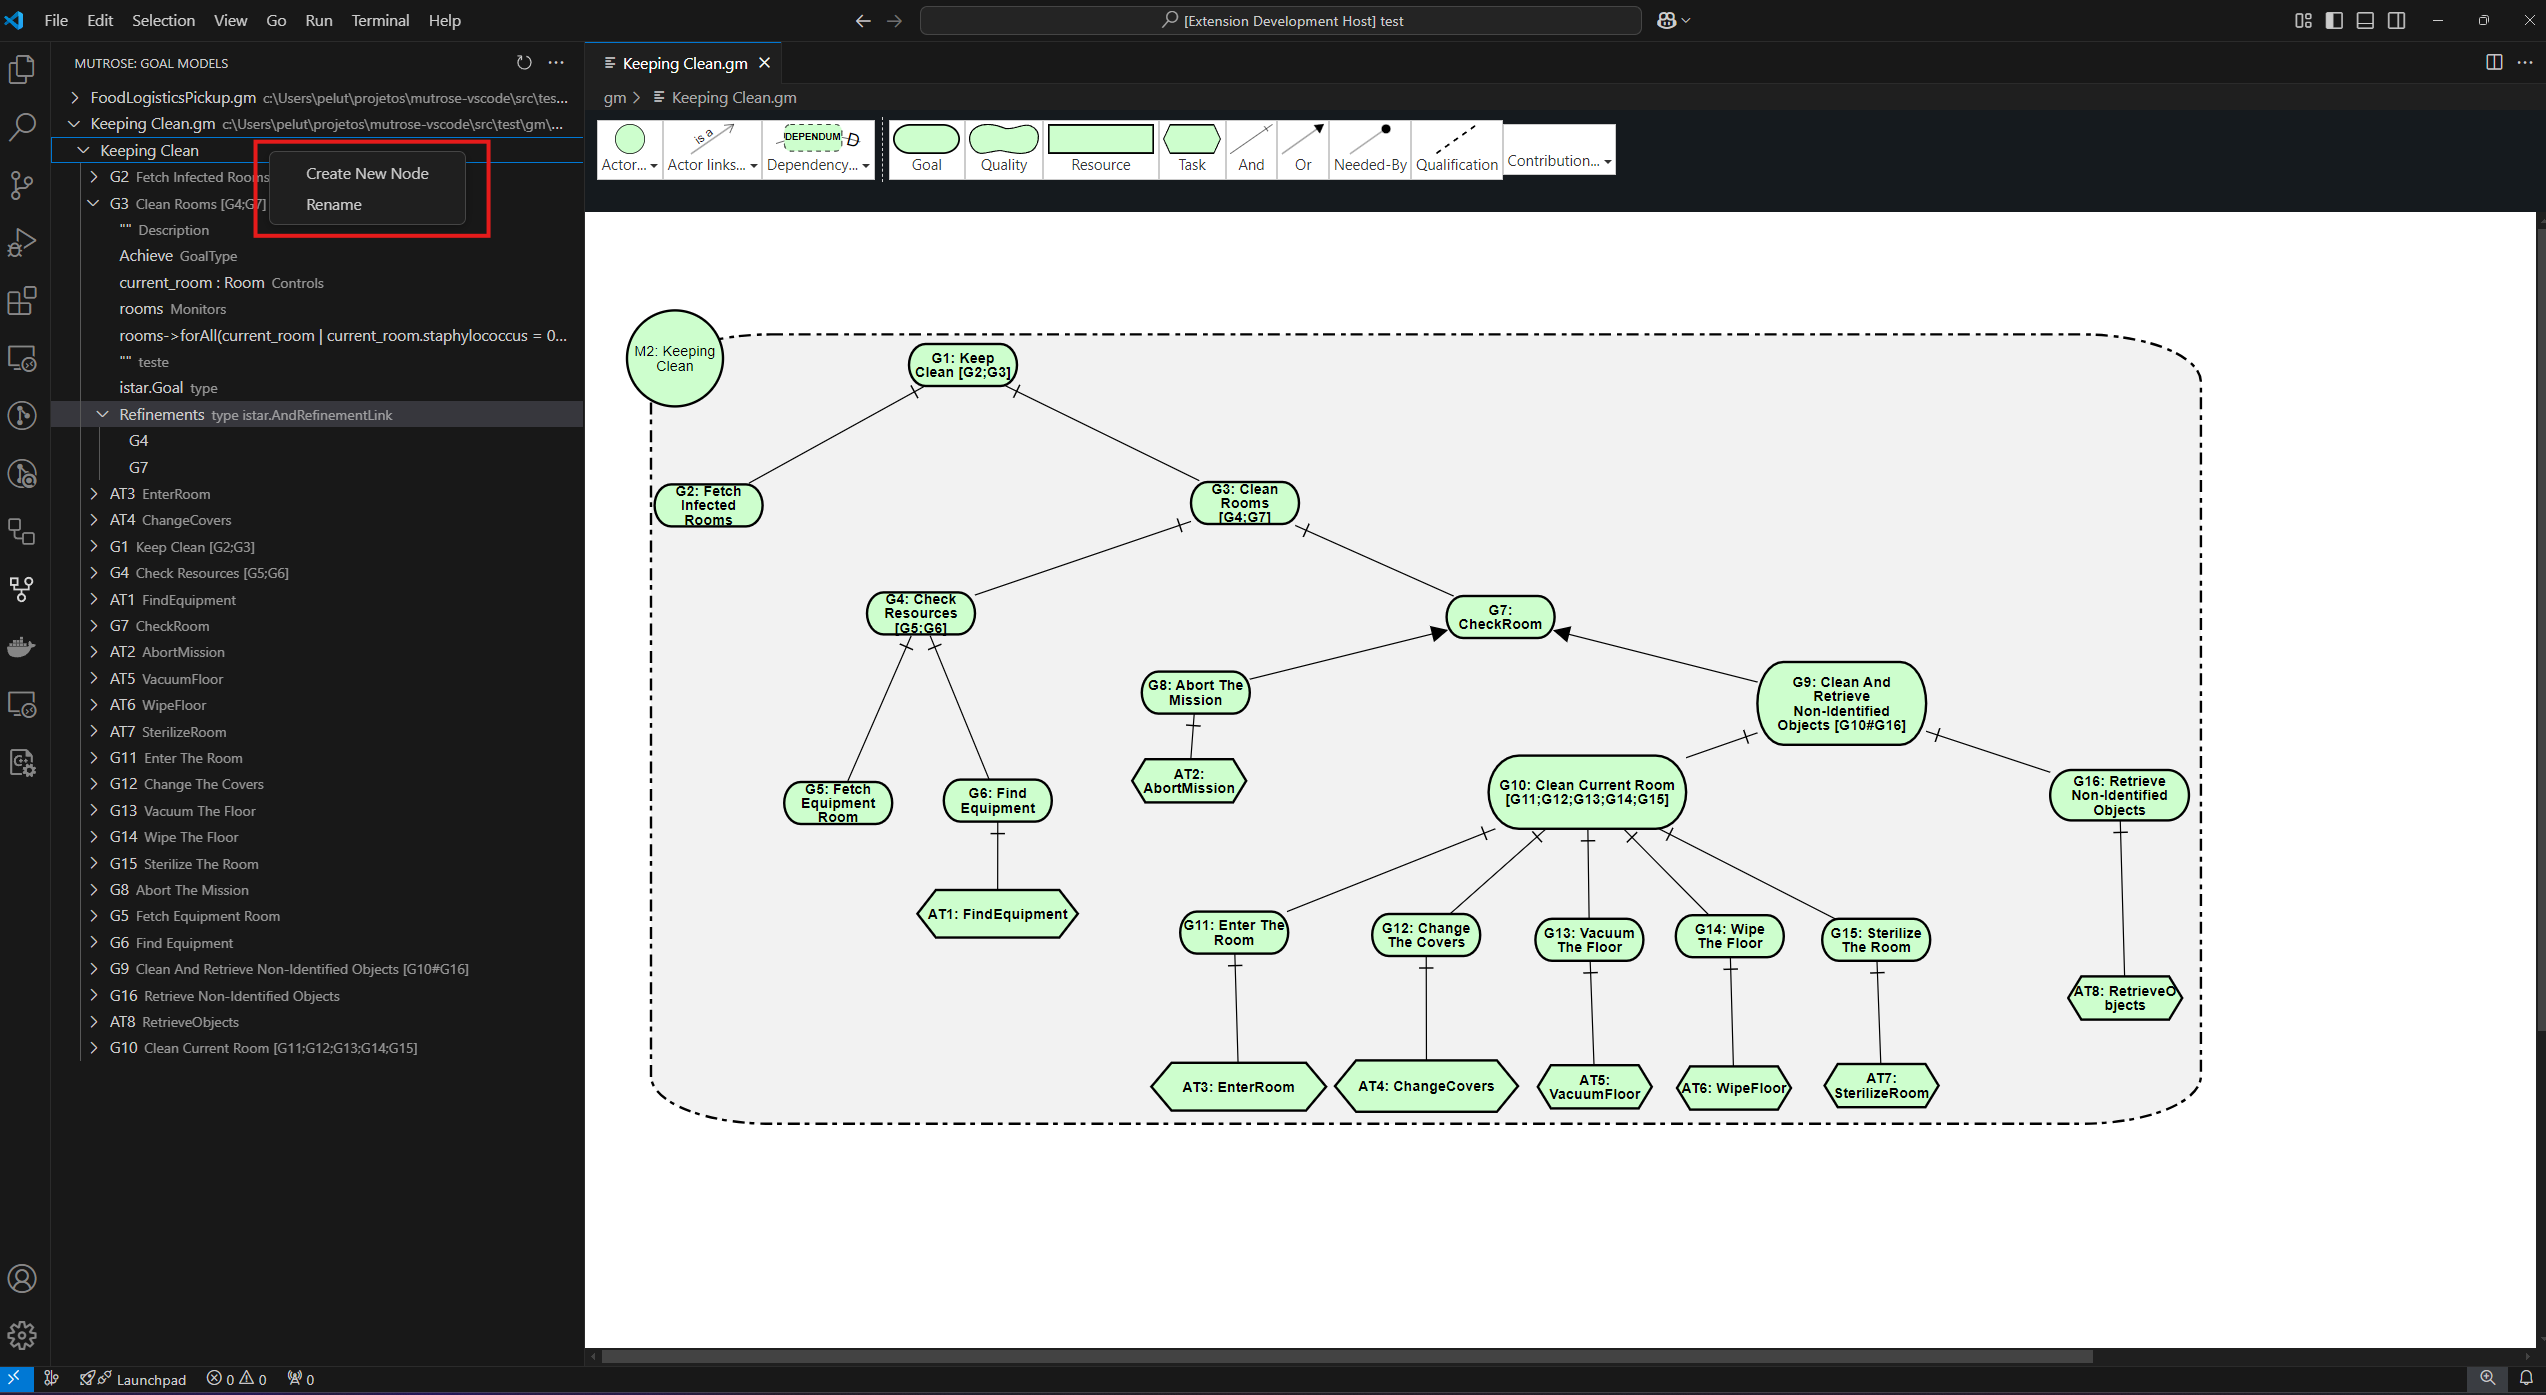
\includegraphics[width=1\textwidth]{rightclickonmission.png} 
    \caption{}
  \end{figure}
\end{frame}
\begin{frame}{Exemplo de fluxo}
  \begin{figure}[!h]
    \centering
    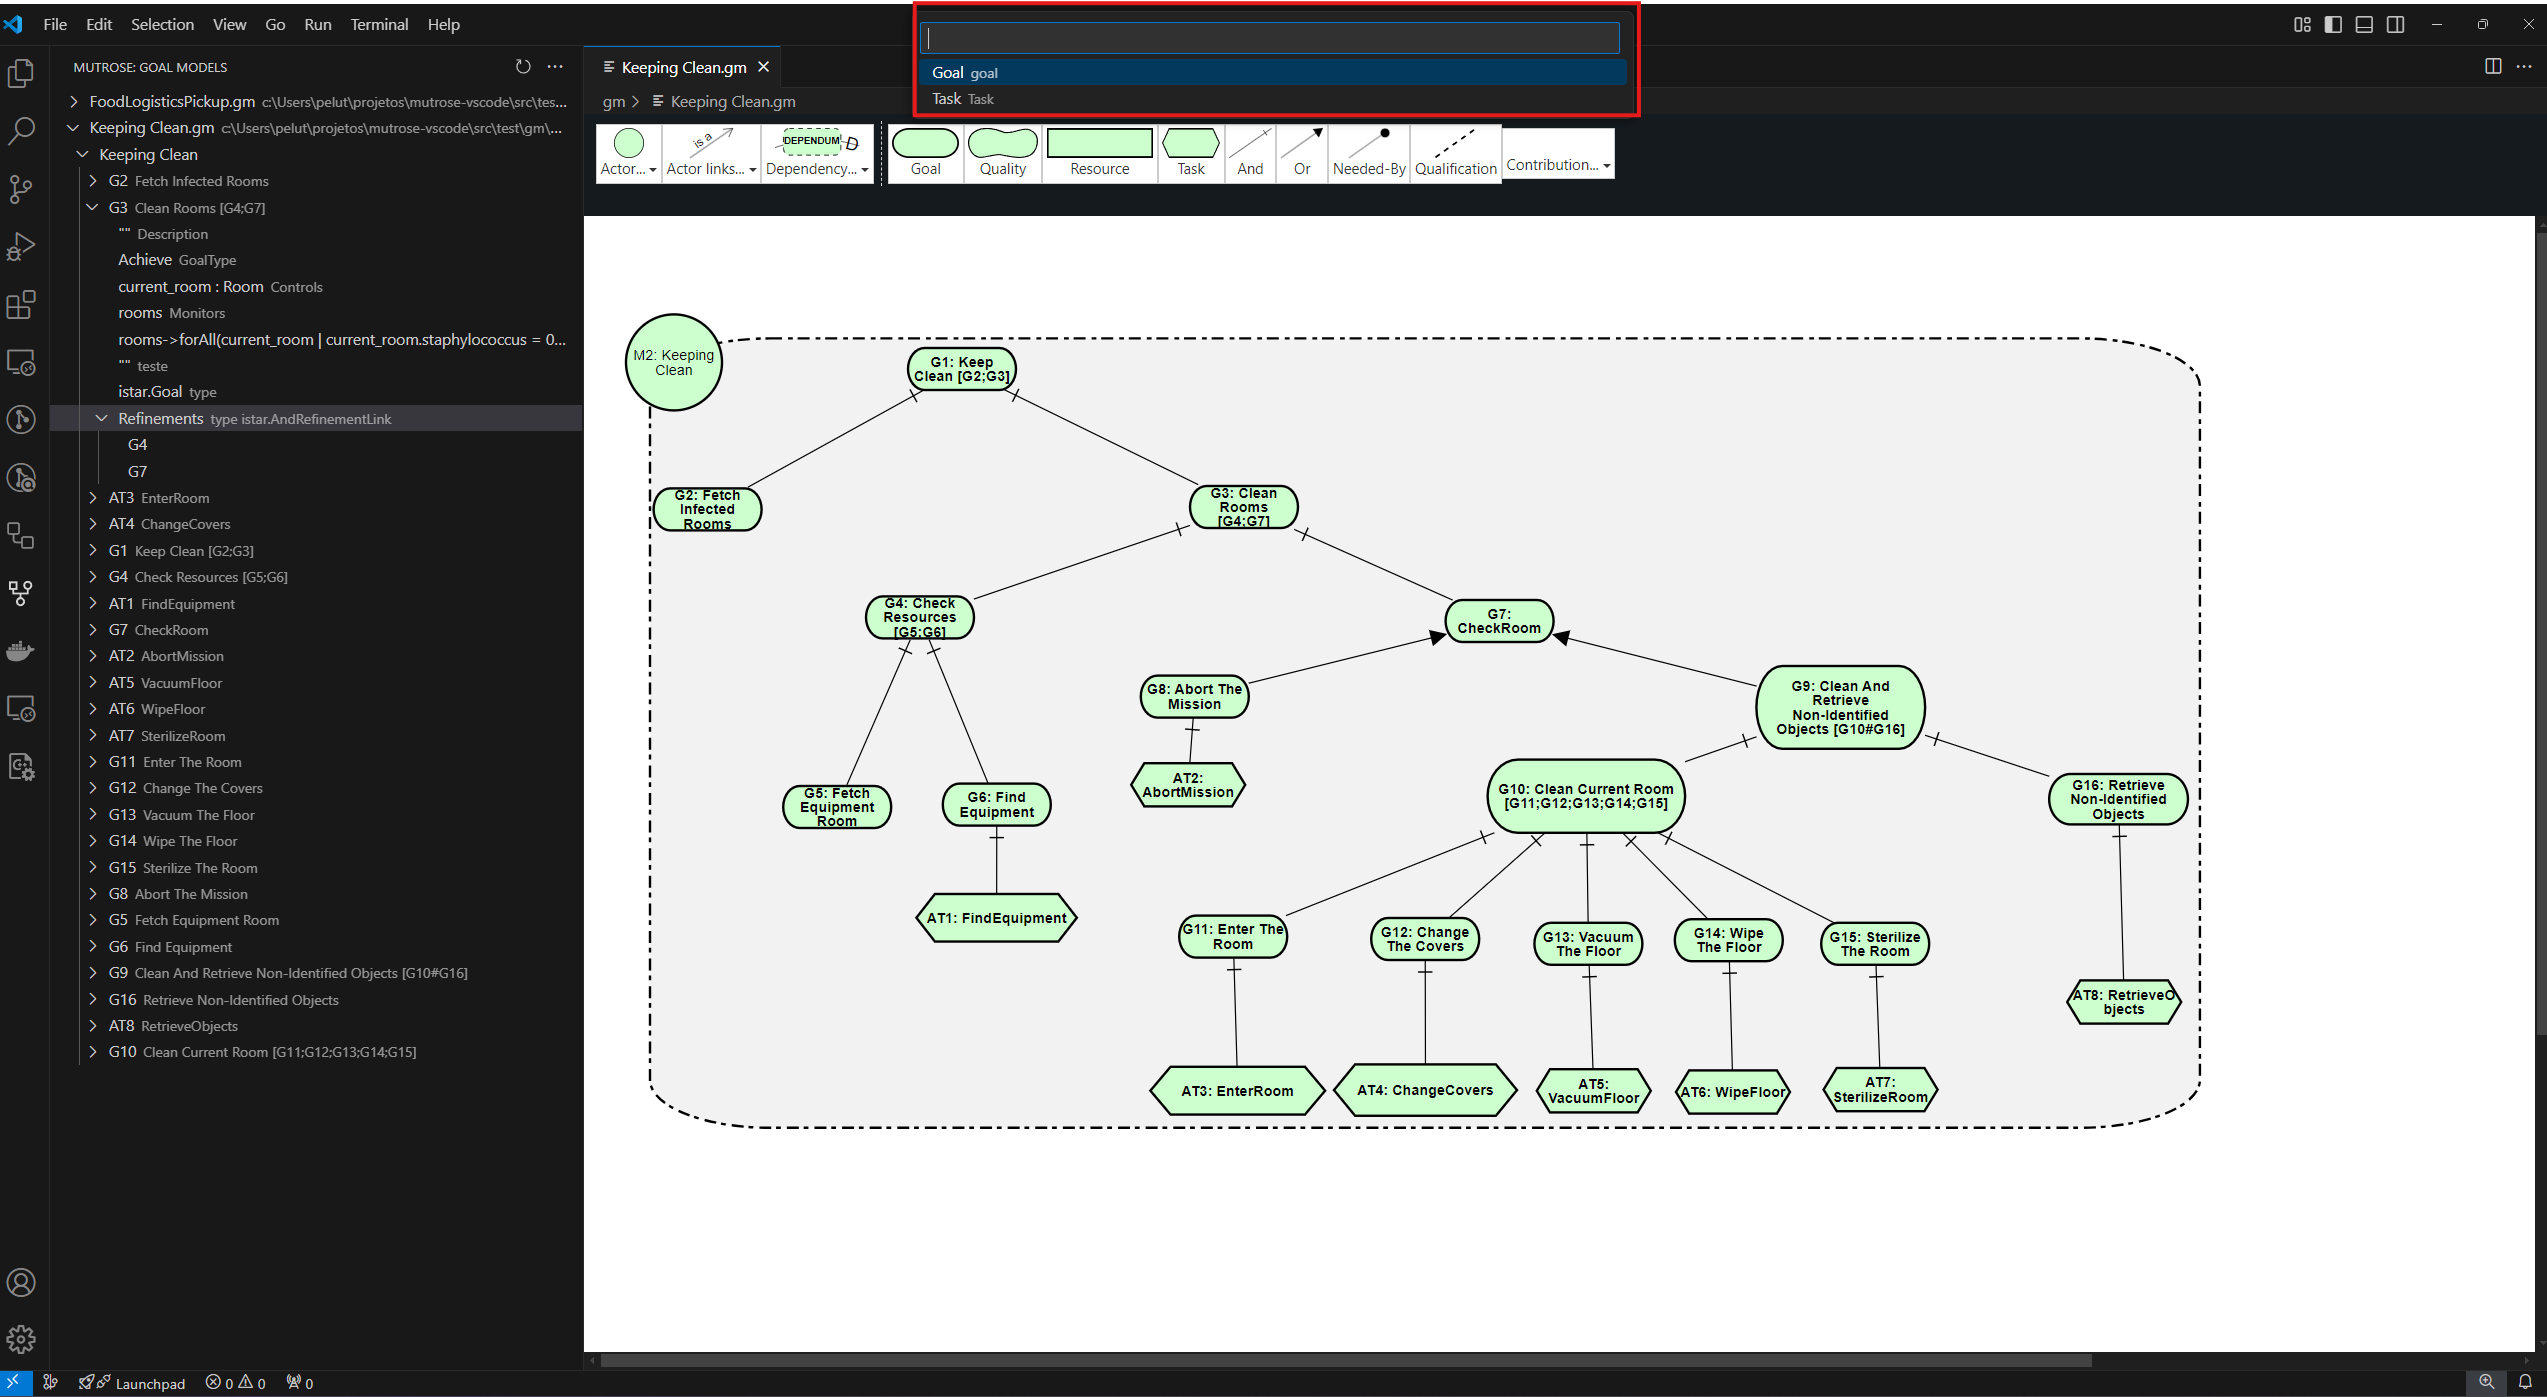
\includegraphics[width=1\textwidth]{flow1.png} 
    \caption{}
  \end{figure}
\end{frame}
\begin{frame}
  \begin{figure}[!h]
    \centering
    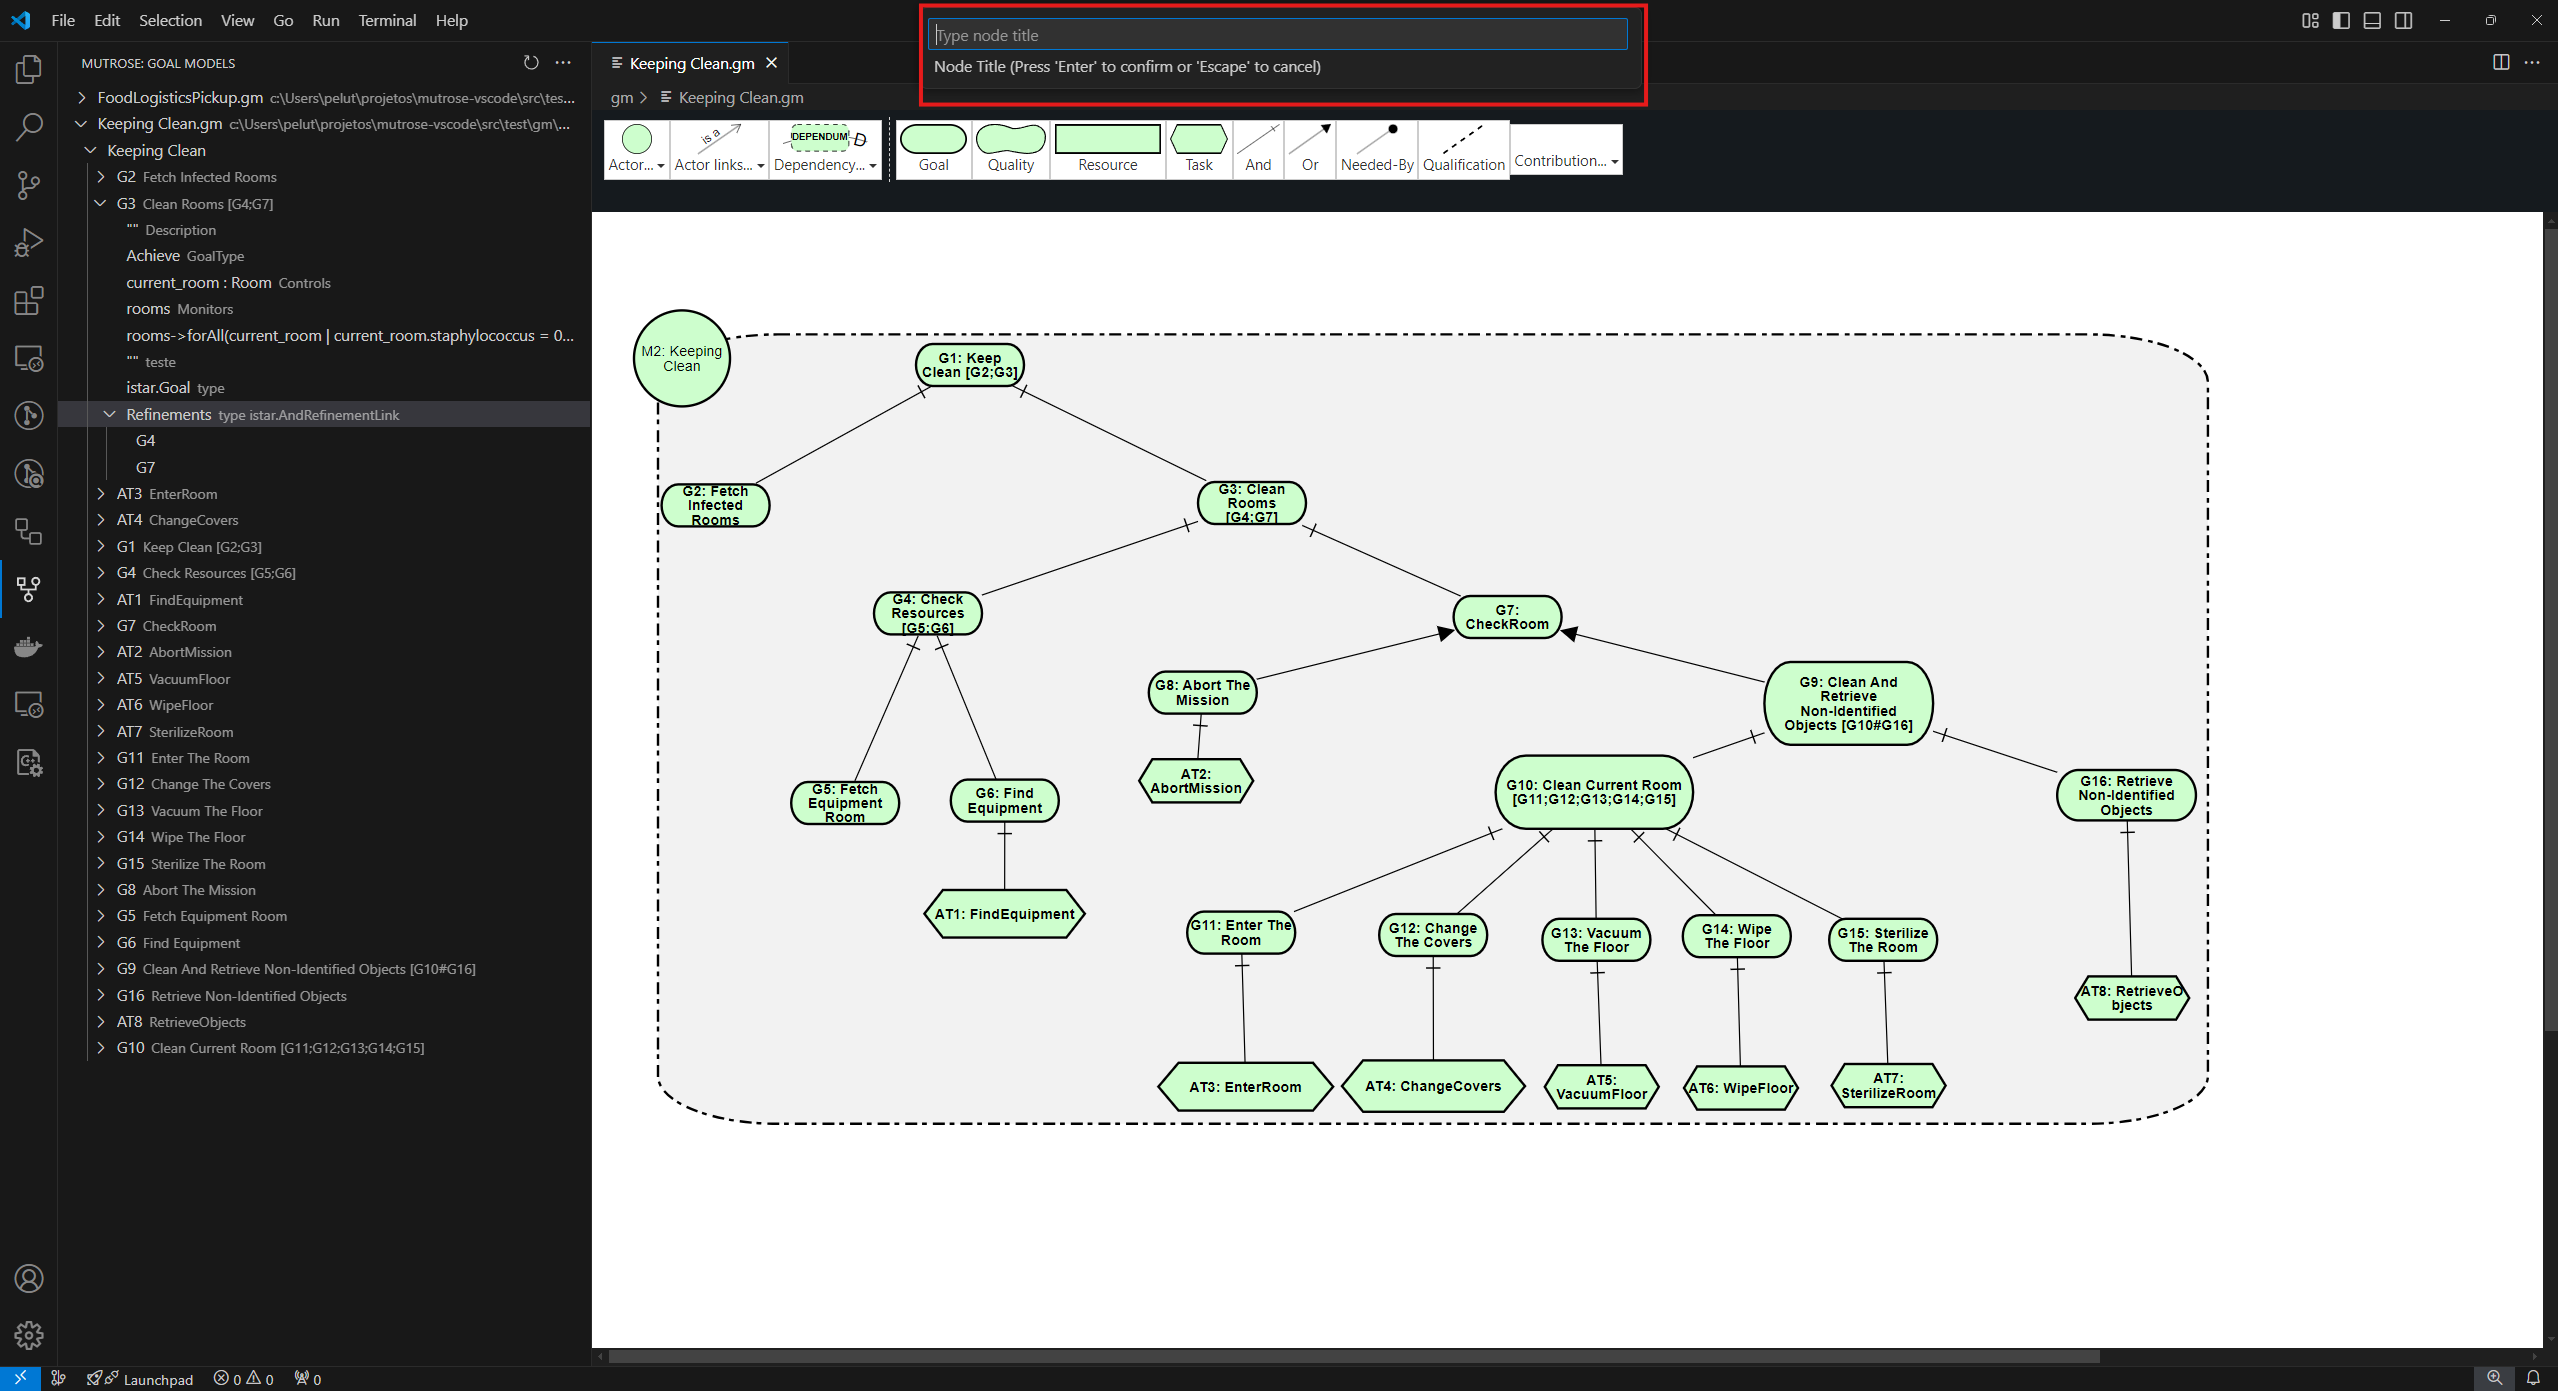
\includegraphics[width=1\textwidth]{flow2.png} 
    \caption{}
  \end{figure}
\end{frame}
\begin{frame}{Executar MutRoSe}
  \begin{figure}[!h]
    \centering
    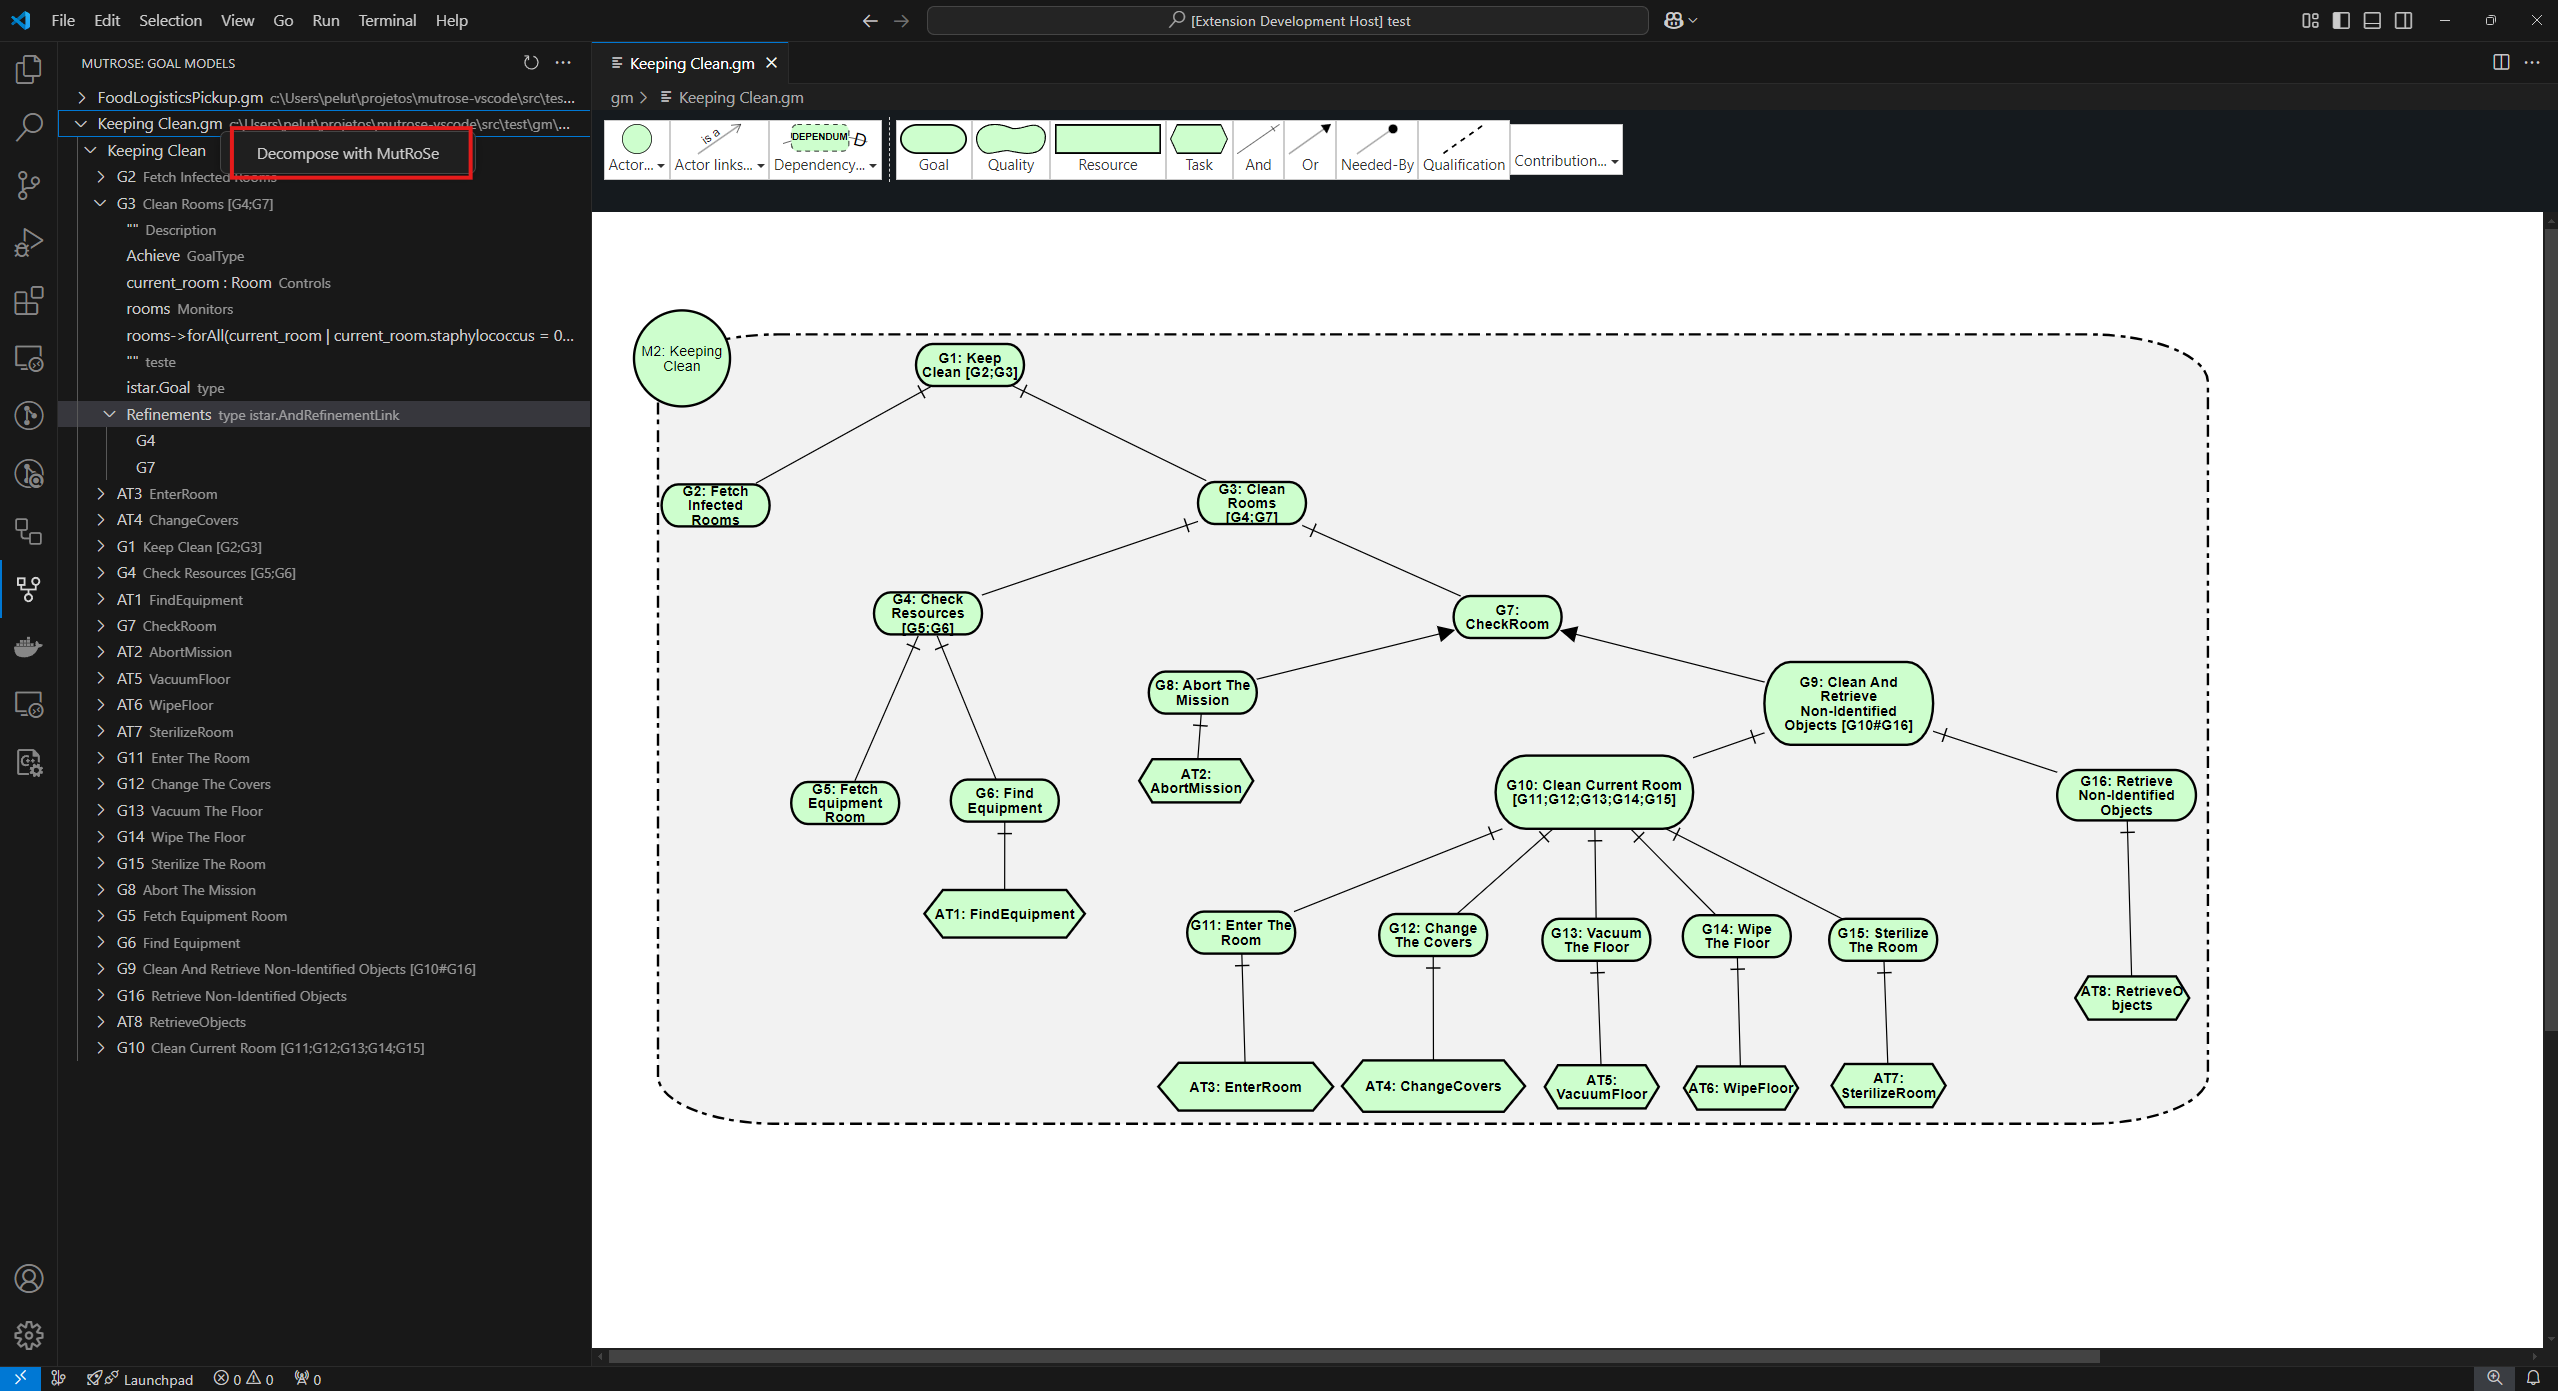
\includegraphics[width=1\textwidth]{decompose.png} 
    \caption{}
  \end{figure}
\end{frame}
\section{Conclusão}
\begin{frame}{Vantagens e Desvantagens}
  \begin{table}[h!]
      \centering
      \begin{tabular}{|p{2cm}|p{4cm}|p{4.5cm}|}
        \hline
        \textbf{Ambientes} & \textbf{Vantagens} & \textbf{Desvantagens} \\
        \hline
        \textbf{Atual} & 
          \begin{itemize}
            \item Já foi testado.
            \item É utilizado como base para diversos projetos.
          \end{itemize}&
          \begin{itemize}
            \item É fragmentado.
            \item Não possui nenhum assistência para detecção de erros.
            \item Não é intuitivo.
          \end{itemize}\\
        \hline
        \textbf{VSCode} & 
          \begin{itemize}
            \item É possível integrar com um Language Server.
            \item É centralizado.
            \item É possível definir um fluxo de modelagem.
          \end{itemize}&
          \begin{itemize}
            \item É dependente do VSCode.
            \item Utiliza a API de TreeView do VSCode.
            \item Ainda não foi testado.
          \end{itemize}\\
        \hline
      \end{tabular}
    \end{table}
      % o que foi, principal cliente
\end{frame}
\begin{frame}{Onde estamos e próximos passos}
  \begin{figure}[!h]
    \centering
    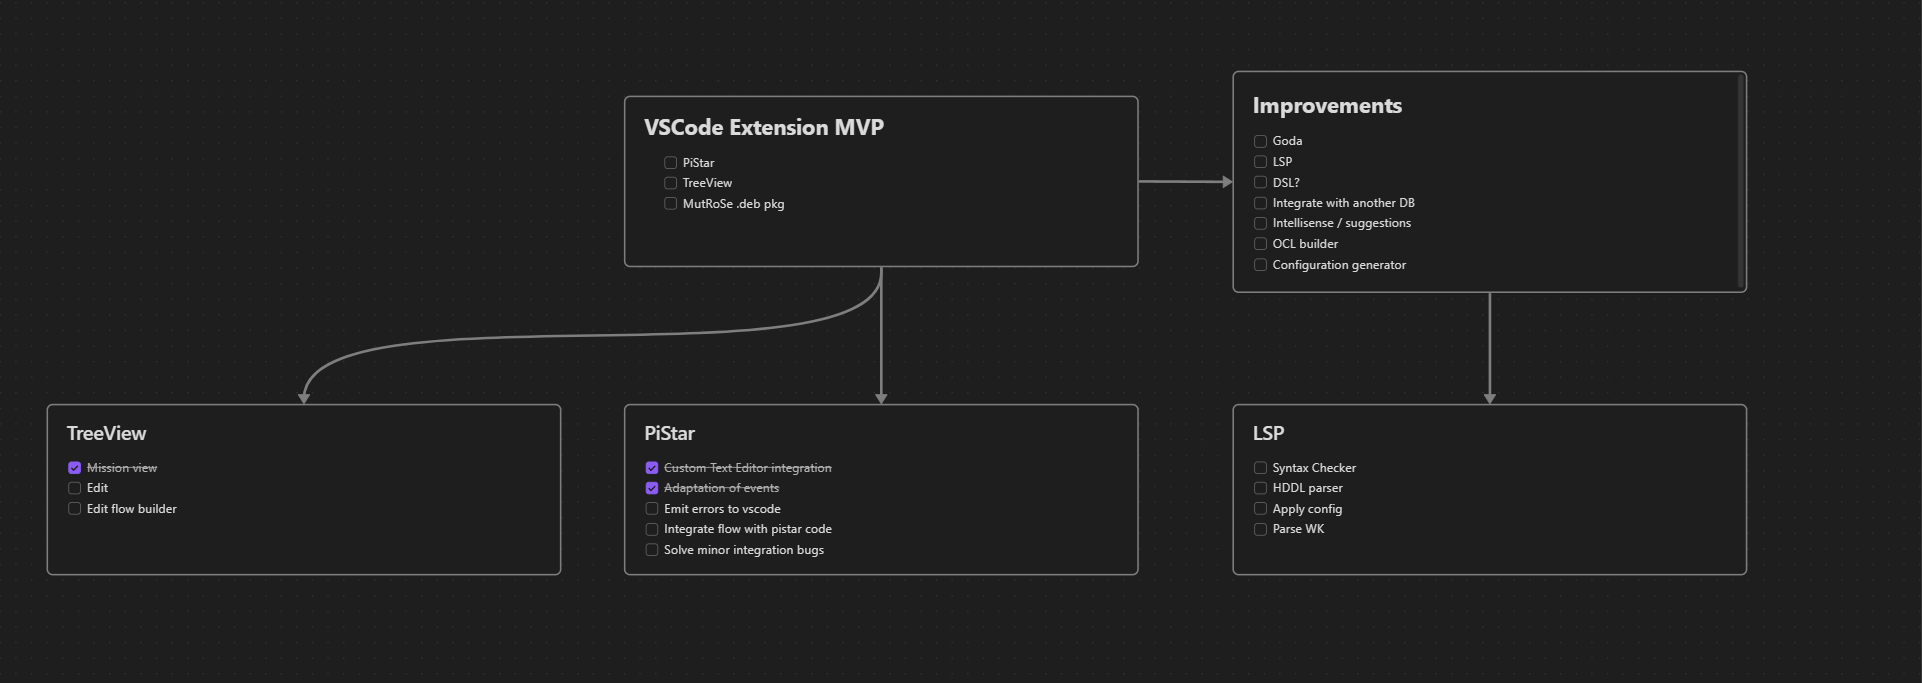
\includegraphics[width=1\textwidth]{VSCode extension.png} 
    \caption{}
  \end{figure}
\end{frame}
\begin{frame}{Exemplo de adições}
  \begin{figure}[!h]
    \centering
    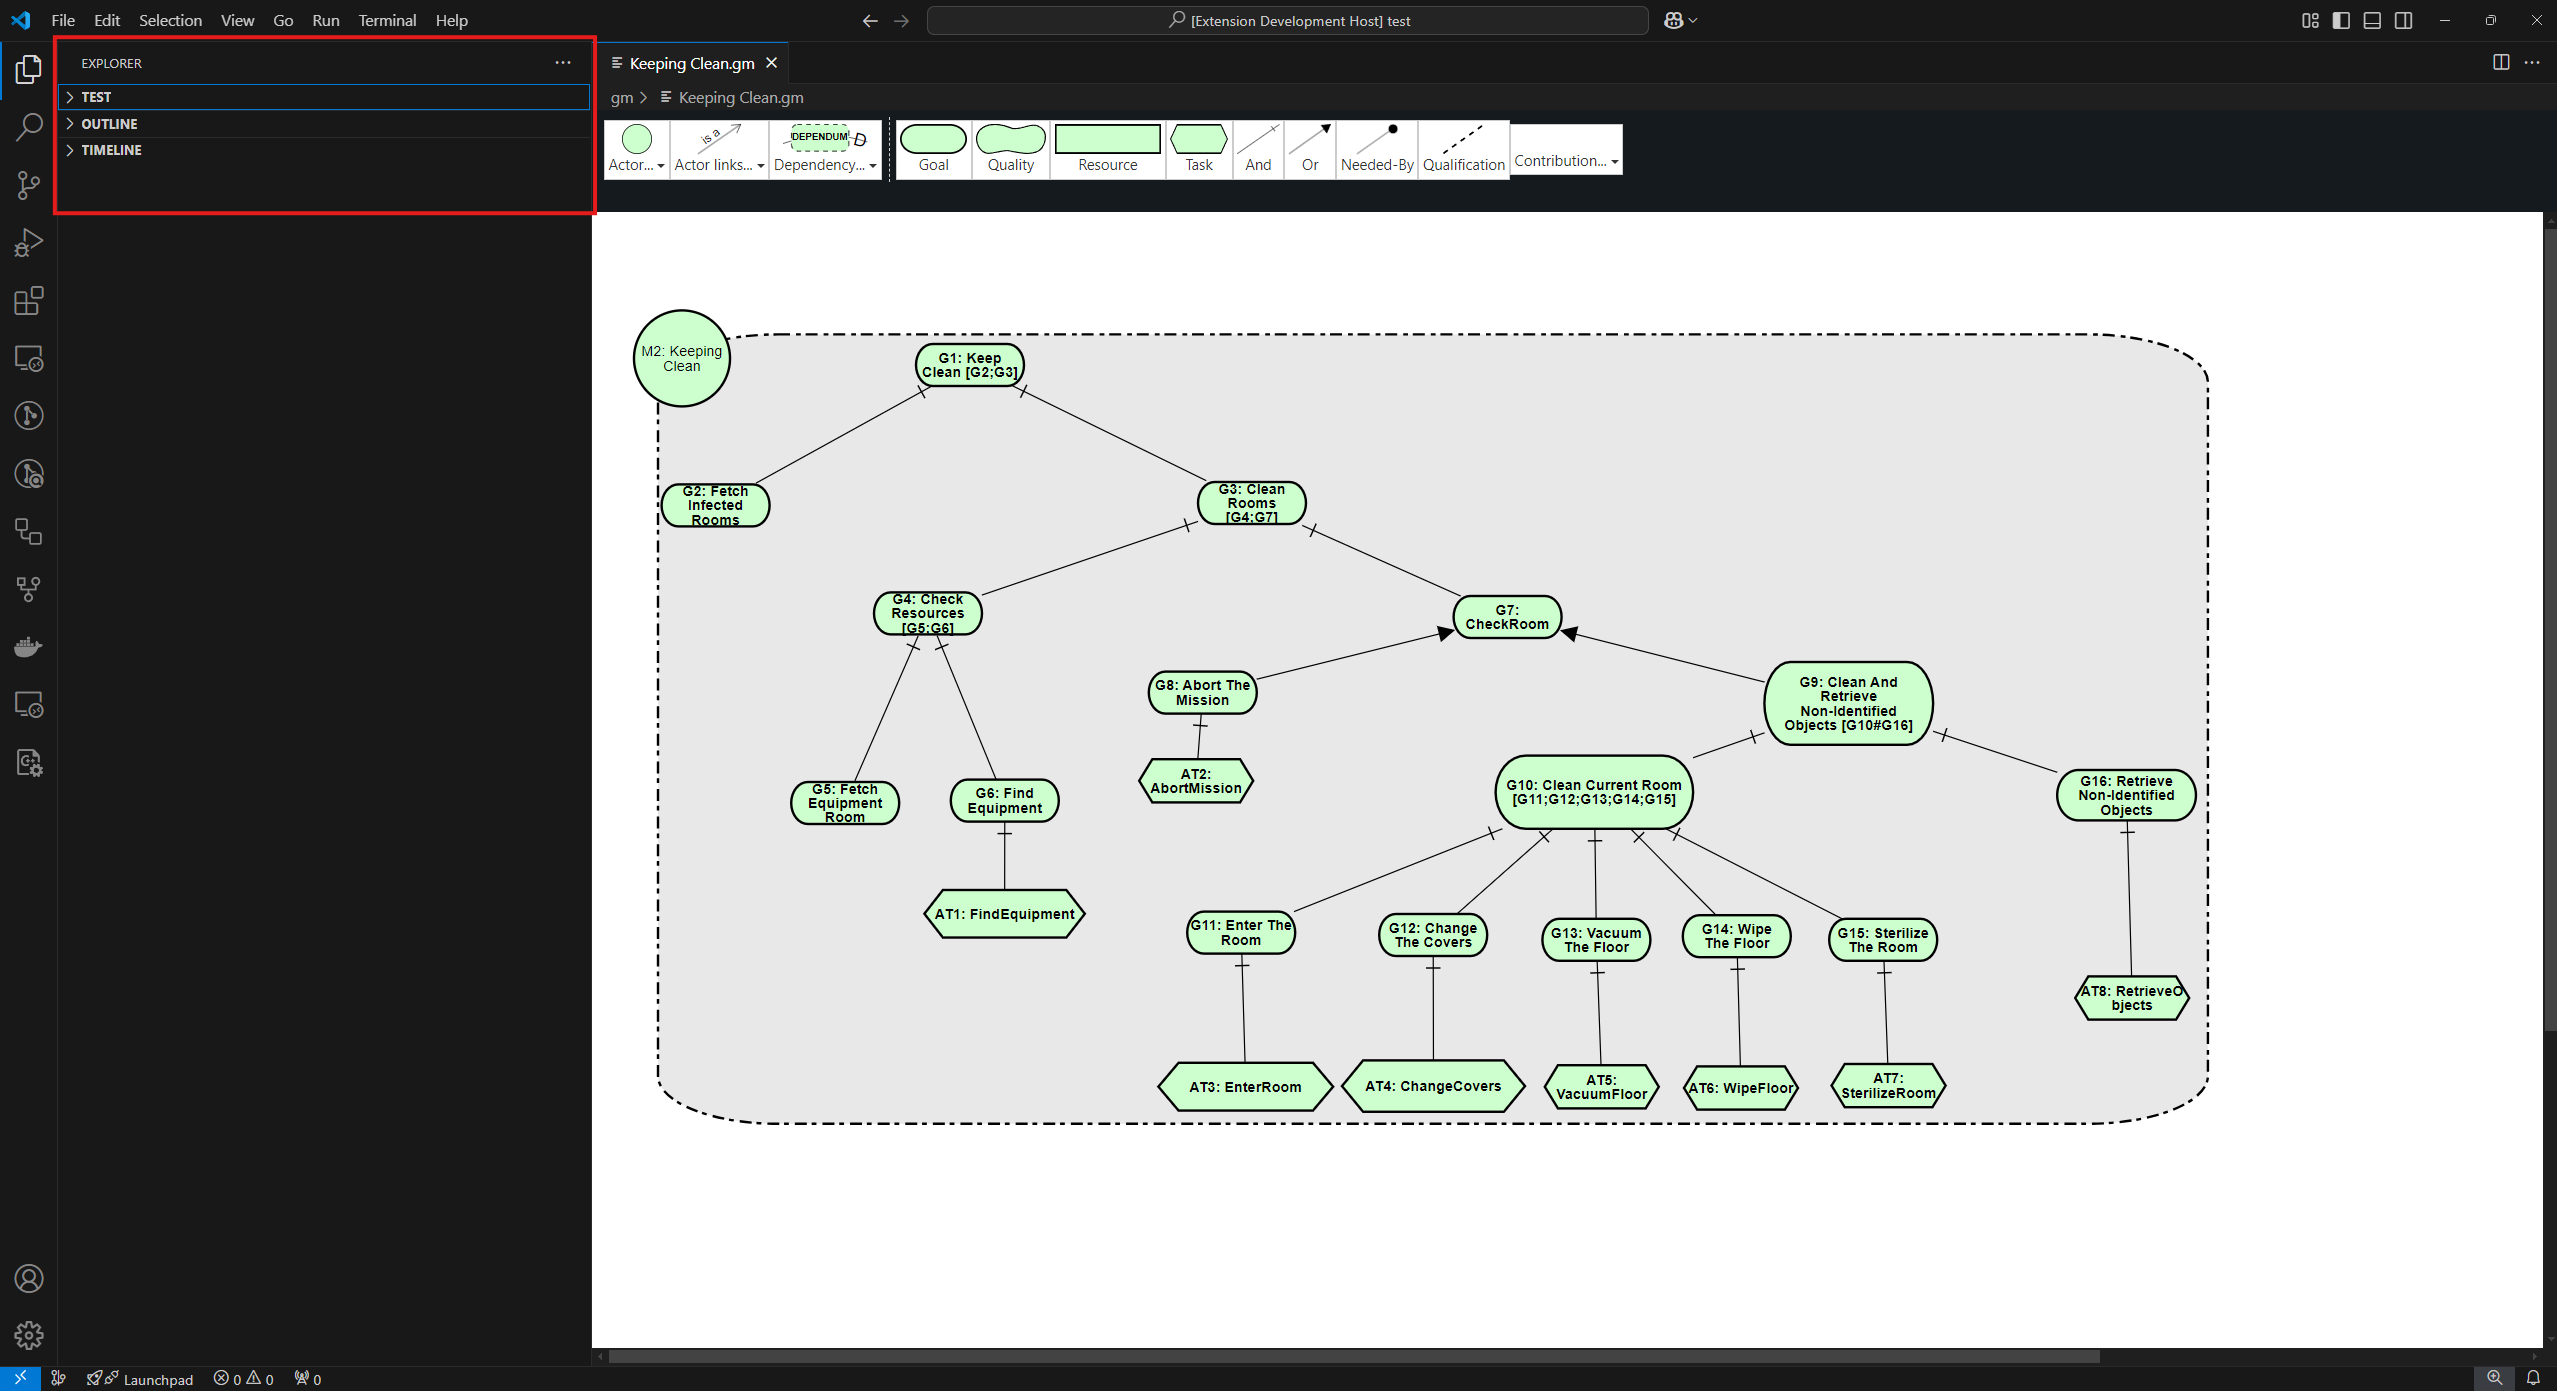
\includegraphics[width=1\textwidth]{multiple sections example.png} 
    \caption{}
  \end{figure}
\end{frame}

% \begin{frame}{Video}
%     \frametitle{Video Example}
%     \includemedia[
%         activate=onclick,
%         width=0.8\textwidth, height=0.6\textheight,
%         addresource=video.mp4,
%         flashvars={source=video.mp4}
%     ]{}{VPlayer.swf}
% \end{frame}


\begin{frame}{}
    \vspace{1cm}\hspace{5cm}\textbf{Obrigado!}
\end{frame}


\end{document}